\documentclass[]{book}
\usepackage{lmodern}
\usepackage{amssymb,amsmath}
\usepackage{ifxetex,ifluatex}
\usepackage{fixltx2e} % provides \textsubscript
\ifnum 0\ifxetex 1\fi\ifluatex 1\fi=0 % if pdftex
  \usepackage[T1]{fontenc}
  \usepackage[utf8]{inputenc}
\else % if luatex or xelatex
  \ifxetex
    \usepackage{mathspec}
  \else
    \usepackage{fontspec}
  \fi
  \defaultfontfeatures{Ligatures=TeX,Scale=MatchLowercase}
    \setmainfont[]{NanumGothic}
\fi
% use upquote if available, for straight quotes in verbatim environments
\IfFileExists{upquote.sty}{\usepackage{upquote}}{}
% use microtype if available
\IfFileExists{microtype.sty}{%
\usepackage{microtype}
\UseMicrotypeSet[protrusion]{basicmath} % disable protrusion for tt fonts
}{}
\usepackage{hyperref}
\hypersetup{unicode=true,
            pdftitle={삽화편두통 예방치료약물 진료지침},
            pdfauthor={대한두통학회 편두통진료지침위원회},
            pdfborder={0 0 0},
            breaklinks=true}
\urlstyle{same}  % don't use monospace font for urls
\usepackage{natbib}
\bibliographystyle{apalike}
\usepackage{longtable,booktabs}
\usepackage{graphicx,grffile}
\makeatletter
\def\maxwidth{\ifdim\Gin@nat@width>\linewidth\linewidth\else\Gin@nat@width\fi}
\def\maxheight{\ifdim\Gin@nat@height>\textheight\textheight\else\Gin@nat@height\fi}
\makeatother
% Scale images if necessary, so that they will not overflow the page
% margins by default, and it is still possible to overwrite the defaults
% using explicit options in \includegraphics[width, height, ...]{}
\setkeys{Gin}{width=\maxwidth,height=\maxheight,keepaspectratio}
\IfFileExists{parskip.sty}{%
\usepackage{parskip}
}{% else
\setlength{\parindent}{0pt}
\setlength{\parskip}{6pt plus 2pt minus 1pt}
}
\setlength{\emergencystretch}{3em}  % prevent overfull lines
\providecommand{\tightlist}{%
  \setlength{\itemsep}{0pt}\setlength{\parskip}{0pt}}
\setcounter{secnumdepth}{5}
% Redefines (sub)paragraphs to behave more like sections
\ifx\paragraph\undefined\else
\let\oldparagraph\paragraph
\renewcommand{\paragraph}[1]{\oldparagraph{#1}\mbox{}}
\fi
\ifx\subparagraph\undefined\else
\let\oldsubparagraph\subparagraph
\renewcommand{\subparagraph}[1]{\oldsubparagraph{#1}\mbox{}}
\fi

%%% Use protect on footnotes to avoid problems with footnotes in titles
\let\rmarkdownfootnote\footnote%
\def\footnote{\protect\rmarkdownfootnote}

%%% Change title format to be more compact
\usepackage{titling}

% Create subtitle command for use in maketitle
\providecommand{\subtitle}[1]{
  \posttitle{
    \begin{center}\large#1\end{center}
    }
}

\setlength{\droptitle}{-2em}

  \title{삽화편두통 예방치료약물 진료지침}
    \pretitle{\vspace{\droptitle}\centering\huge}
  \posttitle{\par}
    \author{대한두통학회 편두통진료지침위원회}
    \preauthor{\centering\large\emph}
  \postauthor{\par}
      \predate{\centering\large\emph}
  \postdate{\par}
    \date{2019-06-27}

\usepackage{booktabs}
\usepackage{amsthm}

% Landscape
%l\usepackage{lscape}
%\newcommand{\blandscape}{\begin{landscape}}
%\newcommand{\elandscape}{\end{landscape}}

\makeatletter
\def\thm@space@setup{%
  \thm@preskip=8pt plus 2pt minus 4pt
  \thm@postskip=\thm@preskip
}
\makeatother

\begin{document}
\maketitle

{
\setcounter{tocdepth}{1}
\tableofcontents
}
\frontmatter

\hypertarget{section}{%
\chapter*{머리말}\label{section}}
\addcontentsline{toc}{chapter}{머리말}

This is preface.

\hypertarget{section-1}{%
\chapter*{발간사}\label{section-1}}
\addcontentsline{toc}{chapter}{발간사}

\textbf{삽화편두통 예방치료약물''에 대한 임상진료지침 발간을 축하하며}

우선 본 지침을 만들기 위해 노고를 아끼지 않으신 총괄책임자인 정재면위원장님과 모든 실무를 도맡아 해주신 박광열간사님을 비롯한 참여하여 주신 모든 분들께 학회를 대표하여 깊은 감사의 말씀을 드립니다.

편두통은 가장 흔한 뇌질환으로 전세계 13억 인구가 고통받고 있습니다. 흔할 뿐아니라 반복되는 통증과 두통에 동반된 증상들로 인한 장애도 매우 커서 세계보건기구(WHO)의 조사에서 질병부담이 큰 질환 2위일 정도로, 심각하게 환자의 삶의 질을 저하시키고 사회경제적 비용 부담을 유발하는 질환입니다. 하지만 아직 편두통에 대한 의과대학과정이나 수련과정에서 교육시간은 절대 부족하고 사회와 보건당국의 이해와 관심은 미미하여 전체 편두통환자의 10\% 미만이 제대로 진단과 치료를 받고 있습니다.

최근 편두통의 중요성이 부각됨에 따라 미국과 유럽의 많은 나라에서 앞다투어 편두통 진료지침을 제시하고 있습니다. 하지만 편두통의 치료의 많은 부분이 근거보다는 전문가의 견해에 의존하고 있고 나라마다 허가된 약제들이 다르기 때문에 다양한 진료지침은 때로는 혼란의 원인이 될 수도 있습니다. 그런 만큼 우리나라 현실에 부합하고 일차 진료현장에서 쉽게 적용할 수 있는 가이드라인을 개발하여 활용할 필요성이 어느 때보다 높다고 생각합니다. 과거 두차례 대한두통학회의 편두통진료지침이 있었지만 본 지침서는 대한의학회의 진료지침의 개발과 평가방법에 맞춘 최초의 체계적인 임상진료지침이라는 큰 의의가 있습니다.

본 진료지침은 세계 주요 국가에서 사용되고 있는 진료지침들을 분석하여 우리나라 의료 현장에 맞게 조정하였고, 본 학회 이외도 진료지침 전문가의 자문을 받아 더욱 완성도를 높였습니다. 편두통 치료에 있어 신기원을 이루는 새로운 약제와 기구들이 수년 내에 국내 출시 예정입니다. 빠른 시일내에 새로 개발된 치료법을 포함하는 새로운 지침서를 기대합니다.

\textbf{대한두통학회 회장 김병건}

\hypertarget{section-2}{%
\chapter*{간행사}\label{section-2}}
\addcontentsline{toc}{chapter}{간행사}

대한두통학회 창립 20주년을 맞이하여 삽화편두통 예방치료약물 진료지침이 발간됩니다. 삽화편두통의 예방치료약물에 관한 표준진료지침 개발의 개시모임이 2016년 11월 21일 이었으므로 벌써 2년 반의 시간이 흘렀습니다. 외국에서 발간된 진료지침에 의존하여 두통 환자를 치료해 오던 것을 탈피하여 우리 두통학회의 힘으로 온전히 우리나라 임상현실에 근거한 두통 관련 진료지침을 개발하기로 마음을 모은 날입니다.
이미 2002년 우리 두통학회에서는 편두통진료지침이 발간된 바 있습니다. 하지만 내용적으로는 두통학회 이사진이 당시 미국 신경과학회에서 발간된 ``Practice guideline for migraine headache''를 발췌 번역하고, 수록된 편두통 치료약물 중에서 우리나라에서 사용되고 있는 약물을 정리하여 발간한 것이었습니다. 우리의 임상 상황과는 상이한 부분이 있었고, 건강보험 체계 등의 현실이 반영되지 않았다는 점에서 진정한 우리나라의 진료지침으로 받아들여지기에는 부족한 점이 많았습니다. 2000년대에 들어서 국내의 여러 임상학회에서 근거중심의학에 기반한 다양한 표준진료지침 개발의 움직임이 일어나 많은 임상의학 영역에서 표준진료지침이 속속 발표되었습니다. 우리 두통학회에서도 2009년 제1판 편두통 진료지침이 개발된 이후 새롭게 발표된 근거를 추가 보완하여 편두통 진료지침 제2판(이광수 회장, 정성우 위원장)을 발간하였습니다. 제2판에는 소아 편두통의 약물치료에 대한 새로운 지침을 추가하였다는 의미가 크다고 할 수 있겠습니다. 하지만 내용적으로는 우리나라의 임상현실을 충분히 반영하지 못한 아쉬움이 있었습니다. 이후 진료지침 개발에 대한 방법론적인 발전을 토대로 한 진료지침이 다양한 임상영역에서 개발되기 시작하였습니다. 여기에는 대한의학회의 지원, 2009년 NECA(한국보건의료연구원)의 개원으로 이루어진 체계적인 기술지원이라는 배경이 있습니다. 이에 대한신경과학회에서도 표준진료지침위원회(위원장 김원주교수, 연세대)를 신설하고 신경과 영역에서 진료지침 개발을 서두르게 되었습니다. 마침 비슷한 뜻을 가지고 진료지침 개발의 필요성을 절감하고 정도관리위원회(위원장 정재면교수, 인제대)를 신설하여 준비 중이던 대한두통학회가 동참하기로 결정하였습니다. 대한신경과학회의 김원주 이사, 대한두통학회 김병건 회장, 정재면 이사 외에 간사로 박광열 교수(중앙대), 위원으로 김병수 선생(분당재생병원), 서종근 교수(경북대), 손종희 교수(한림대), 송태진 교수(이화여대), 이미지 교수(성균관대), 정필욱 교수(성균관대), 최윤주 선생(전주예수병원) 등이 참여하게 되었습니다. 진료지침의 기술적인 자문을 위해 NECA의 박동아 선생이 참여하게 되었습니다.

2016년 11월 21일 개시모임에서 경험이 일천한 우리 학회의 입장을 고려하여 가능한 한 진료지침의 범위를 좁게 하고 문헌고찰의 부담을 작게 하기 위해 편두통의 치료 가운데 삽화편두통의 예방치료약물로 범위를 한정하였고, 개발방식에 있어서도 2012년 이후 발표된 해외 진료지침 중 영어로 기술되어 있고 다학제 참여가 이루어지고 근거에 기반한 진료지침을 선정하여 Hybrid 방식으로 개발하기로 하였습니다. 표준진료지침의 가장 중요한 핵심질문은 실무위원들의 논의를 거쳐 7가지로 정하게 되었습니다. 이후 수 차례의 회의와 작업을 거쳐 핵심질문에 관한 내용을 담고 있는 외국 진료지침을 AGREE II 도구를 이용하여 평가한 후 총 9개의 진료지침이 선정되었습니다. 9개의 진료지침을 토대로 최신성 검색을 통해 새로운 근거에 대한 검토가 이루어지게 되었습니다. 이러한 과정에서 겪게되는 기술적인 어려움을 극복하기 위해 대한의학회에서 개최하는 진료지침 개발 워크샵에 위원장과 간사를 포함해 위원들이 적극적으로 참여하여 지식과 경험을 넓혀 갔습니다. 우리학회 나름대로도 진료지침 전문가인 순천향대학교 이유경 교수를 초청하여 강의와 토의를 통해 임상의사의 입장에서 진료지침의 전문성을 높이기 위한 노력이 있었습니다. 최신성 검토를 위해 문헌을 검색하여 자료를 추출하는 어려운 작업은 NECA의 최미영 연구위원이 맡아주는 등 많은 분들의 도움이 있었습니다. 이번 기회를 빌어 외부인사들께 감사의 마음을 전합니다.

이런 일련의 작업들을 통해 진료지침의 근거가 마련이 되었습니다. 어떤 예방약물을 어떤 권고의 수준으로 결정하느냐 하는 문제는 단순히 근거가 되는 임상시험 결과만을 가지고 결정할 수 없는 문제입니다. 이러한 결정은 우리나라 편두통 환자의 진료형태를 결정할 수도 있는 중요한 문제이기 때문에 실무위원들과 이사진들이 다양한 의견을 나누고 수렴하는 과정을 거쳐 매우 신중하게 진행되었습니다.

우리 대한두통학회 창립 20주년을 맞이하여 이제 근거중심의학에 기반한 제대로 된 두통 표준진료지침의 첫걸음을 내딛게 되었습니다. 완성도에서는 아직도 미흡한 점이 많습니다. 하지만 앞으로 개발될 일련의 두통 관련 표준진료지침들과 후속 개정작업을 통해 우리나라 임상의사들의 두통질환의 진료와 연구 수준을 높이는 계기가 된다는 점에서 그 의미가 크다고 할 수 있겠습니다.

그동안 열정을 잃지 않고 꼼꼼하게 작업을 챙기고 격려해 주신 대한신경과학회 정진상 이사장님과 대한두통학회 김병건 회장님께 감사 드립니다. 고독하고 어려운 일들을 묵묵히 맡아주신 박광열 교수님과 여러 위원들께 다시 한 번 심심한 감사를 드립니다.

\textbf{대한두통학회 편두통진료지침위원장 정재면}

\mainmatter

\hypertarget{section-3}{%
\chapter{요약}\label{section-3}}

\hypertarget{section-4}{%
\section{핵심질문과 권고사항}\label{section-4}}

1. 성인 삽화편두통 환자에서 예방치료를 고려해야 하는 요인들(두통빈도, 두통강도, 환자의 선호도, 일상생활에 대한 영향 등)은 무엇인가?

\begin{itemize}
\item
  삽화편두통에서 생활습관개선과 편두통 급성기치료를 적절하게 시도하였음에도 불구하고 편두통으로 인하여 의미 있는 일상생활의 장애\footnote{두통으로 인한 일상생활의 의미있는 장애(headache-related disability)

    신체적, 심리적, 사회경제적인 측면을 모두 포함하여 두통 환자가 겪게 되는 일상생활의 장애를 포괄적으로 의미하는 것이다. 즉, 두통으로 인한 신체적인 고통, 불안 또는 우울 등의 심리적 반응, 사회경제적인 비용의 증가, 학업 및 사회활동과 여가활동의 위축 등 삶의 질을 저하시키는 일체의 장애를 말한다. 예를 들면 아래와 같은 것이 있다.

    \begin{enumerate}
    \def\labelenumi{\arabic{enumi}.}
    \tightlist
    \item
      두통 때문에 학교나 직장을 결석 또는 결근(조퇴 또는 양호실에서 휴식)한 적이 있다.
    \item
      두통 때문에 학교나 직장에서 학습능률 또는 업무능력이 절반 이하로 감소한 적이 있다.
    \item
      학교나 직장을 다니지 않는 경우(예: 가정주부, 휴직 또는 퇴직), 두통 때문에 가사를 할 수 없었던 적이 있다.
    \item
      학교나 직장을 다니지 않는 경우(예: 가정주부, 휴직 또는 퇴직), 두통 때문에 가사능률이 절반 이하로 감소했던 적이 있다.
    \item
      두통 때문에 공휴일이나 근무시간 외에 가족활동, 사회활동, 또는 여가활동을 참여하지 못했거나 하였더라도 절반 이상의 불편함을 느낀 적이 있다.
    \end{enumerate}}를 겪는 경우에 예방치료를 권고한다. (근거수준: 전문가의견, 권고등급: 강함)
\item
  편두통환자의 1)두통빈도(월 두통일수)가 적더라도 편두통 급성기치료를 하였을 때 편두통이 효과적으로 치료되지 않거나 두통으로 인한 장애를 경험하는 경우, 2)편두통 급성기치료가 효과적이더라도 두통빈도가 잦은 경우에 예방치료를 권고한다. (근거수준: 전문가의견, 권고등급: 강함)
\item
  편두통환자가 편두통 급성기치료제를 월 10--15일 이상 사용하는 경우에 약물과용두통\footnote{\begin{longtable}[]{@{}lr@{}}
    \toprule
    편두통급성기치료제의 종류 & 약물과용두통 진단기준\tabularnewline
    \midrule
    \endhead
    에르고타민 & 월10일 이상 복용\tabularnewline
    트립탄 & 월10일 이상 복용\tabularnewline
    단순진통제(아세트아미노펜,아세틸살리실산) 또는 비스테로이드항염제(NSAIDs) & 월15일 이상 복용\tabularnewline
    마약성(opioid) 진통제 & 월10일 이상 복용\tabularnewline
    복합진통제 & 월10일 이상 복용\tabularnewline
    여러가지 종류의 약제를 혼용해서 복용하는 경우 & 월10일 이상 복용\tabularnewline
    \bottomrule
    \end{longtable}}의 우려가 있으므로 예방치료를 권고한다. (근거수준: 전문가의견, 권고등급: 강함)
\item
  편두통환자의 두통빈도와 무관하게 편두통환자가 편두통 예방치료를 선호하는 경우이거나 담당의사가 임상적으로 예방치료가 필요하다고 판단하는 경우(예시: 뇌간조짐/반신마비편두통)에 예방치료를 고려할 수 있다. (근거수준: 전문가의견, 권고등급: 약함)
\item
  편두통환자가 편두통 급성기치료의 의학적 금기를 가지고 있는 경우에 예방치료를 고려할 수 있다. (근거수준: 전문가의견, 권고등급: 약함)
\end{itemize}

\begin{center}\rule{0.5\linewidth}{\linethickness}\end{center}

2. 성인 삽화편두통 환자에서 예방치료의 중단은 어떻게 결정해야 하는가?

\begin{itemize}
\item
  삽화편두통에서 예방치료의 효능은 적정용량 혹은 최대내약용량(maximal tolerable dose)으로 적어도 2개월 이상 사용한 후 판단할 수 있다. (근거수준: 전문가의견, 권고등급: 약함)
\item
  예방치료가 효과적인 경우 3개월 이상 치료를 지속한 후 용량을 감량하거나 중단하는 것을 시도할 수 있으며, 예방치료를 유지하는 기간은 두통의 빈도 및 강도 외에도 편두통이 일상 생활에 미치는 영향의 정도에 따라 환자마다 개별적으로 접근하는 것을 제안한다. (근거수준: 전문가의견, 권고등급: 약함)
\item
  예방약물을 감량하거나 중단했을 때 편두통의 빈도가 증가하면 약물 용량을 증량하거나 다시 시작하기를 제안한다. (근거수준: 전문가의견, 권고등급: 약함)
\item
  예방치료의 효능, 부작용 및 순응도를 평가하고 유지기간을 결정하기 위해서는 두통일기 작성을 권고한다. (근거수준: 전문가의견, 권고등급: 강함)
\end{itemize}

\begin{center}\rule{0.5\linewidth}{\linethickness}\end{center}

3. 성인 삽화편두통 환자에서 예방치료로 베타차단제를 사용하는 것이 타약제, 위약 또는 치료하지 않는 것에 비해 두통의 완화에 효과적인가?

\begin{itemize}
\item
  프로프라놀롤은 성인 삽화편두통 환자에서 편두통 예방약제로 사용하는 것을 권고한다. (근거수준: 높음, 권고등급: 강함)
\item
  메토프롤롤은 성인 삽화편두통 환자에서 편두통 예방약제로 사용하는 것을 고려할 수 있다.(근거수준: 높음, 권고등급: 강함)
\item
  아테놀롤은 성인 삽화편두통 환자에서 편두통 예방약제로 사용하는 것을 고려할 수 있다. (근거수준: 보통, 권고등급: 약함)
\item
  나돌롤은 성인 삽화편두통 환자에서 편두통 예방약제로 사용하는 것을 고려할 수 있다. (근거수준: 보통, 권고등급: 약함)
\item
  네비볼롤은 성인 삽화편두통 환자에서 편두통 예방약제로 사용하는 것을 고려할 수 있다. (근거수준: 낮음, 권고등급: 약함)
\item
  비소프롤롤은 성인 삽화편두통 환자에서 편두통 예방약제로 사용하지 않을 것을 제안한다. (근거수준: 전문가의견, 권고등급: 약함)
\item
  핀돌롤은 성인 삽화편두통 환자에서 편두통 예방약제로 사용하지 않을 것을 제안한다. (근거수준: 전문가의견, 권고등급: 약함)
\end{itemize}

\begin{quote}
프로프라놀롤과 나돌롤은 편두통예방치료제로 보험급여 인정기준에 포함되어 있으나 그외 베타차단제는 현재 편두통 보험급여 인정기준에 포함되어 있지 않다.
\end{quote}

\begin{center}\rule{0.5\linewidth}{\linethickness}\end{center}

4. 성인 삽화편두통 환자에서 예방치료로 칼슘통로차단제를 사용하는 것이 타약제, 위약 또는 치료하지 않는 것에 비해 두통의 완화에 효과적인가?

\begin{itemize}
\item
  니카르디핀, 니페디핀, 니모디핀 등은 성인 삽화편두통 환자에서 편두통 예방약제로 사용하지 않을 것을 제안한다. (근거수준: 전문가의견, 권고등급: 약함)
\item
  베라파밀은 성인 삽화편두통 환자에서 편두통 예방약제로 사용하지 않을 것을 제안한다. (근거수준: 전문가의견, 권고등급: 약함)
\item
  플루나리진은 성인 삽화편두통 환자에서 편두통 예방약제로 사용하는 것을 고려할 수 있다. (근거수준: 높음, 권고등급: 약함)
\item
  신나리진은 성인 삽화편두통 환자에서 삼환계 항우울제 및 베타차단제에 효과가 없거나 투여가 어려운 경우 편두통 예방약제로 사용하는 것을 고려할 수 있다. (근거수준: 낮음, 권고등급: 약함)
\end{itemize}

\begin{center}\rule{0.5\linewidth}{\linethickness}\end{center}

5. 성인 삽화편두통 환자에서 예방치료로 안지오텐신수용체차단제(angiotensin receptor blocker)나 안지오텐신전환효소억제제(angiotensin-converting enzyme inhibitor)를 사용하는 것이 타약제, 위약 또는 치료하지 않는 것에 비해 두통의 완화에 효과적인가?

\begin{itemize}
\item
  칸데사르탄은 성인 삽화편두통 환자에서 편두통 예방약제로 사용하는 것을 고려할 수 있다. (근거수준: 보통, 권고등급: 약함)
\item
  리시노프릴은 성인 삽화편두통 환자에서 편두통 예방약제로 사용하는 것을 고려할 수 있다. (근거수준: 낮음, 권고등급: 약함)
\item
  텔미사르탄은 성인 삽화편두통 환자에서 편두통 예방약제로 사용하지 않을 것을 권고한다. (근거수준: 낮음, 권고등급: 강함).
\end{itemize}

\begin{center}\rule{0.5\linewidth}{\linethickness}\end{center}

6. 성인 삽화편두통 환자에서 예방치료로 항우울제를 사용하는 것이 타약제, 위약 또는 치료하지 않는 것에 비해 두통의 완화에 효과적인가?

\begin{itemize}
\item
  아미트리프틸린은 성인 삽화편두통 환자에서 편두통 예방약제로 사용하는 것을 권고한다. (근거수준: 보통, 권고등급: 강함)
\item
  벤라팍신은 성인 삽화편두통 환자에서 편두통 예방약제로 사용하는 것을 고려할 수 있다. (근거수준: 보통, 권고등급: 약함)
\item
  플루옥세틴은 성인 삽화편두통 환자에서 편두통 예방약제로 사용하지 않을 것을 제안한다. (근거수준: 매우낮음, 권고등급: 약함)
\item
  노르트리프틸린은 성인 삽화편두통 환자에서 편두통 예방치료제로 사용하는 것을 고려할 수 있다. (근거수준: 매우낮음, 권고등급: 약함)
\end{itemize}

\begin{center}\rule{0.5\linewidth}{\linethickness}\end{center}

7. 성인 삽화편두통 환자에서 예방치료로 뇌전증약을 사용하는 것이 타약제, 위약 또는 치료하지 않는 것에 비해 두통의 완화에 효과적인가?

\begin{itemize}
\item
  토피라메이트는 성인 삽화편두통 환자에서 편두통 예방약제로 사용할 것을 권고한다. (근거수준: 높음, 권고등급: 강함)
\item
  디발프로엑스나트륨은 성인 삽화편두통 환자에서 편두통 예방약제로 사용할 것을 권고한다. 단, 체중 증가, 다낭성 난소 증후군 등의 부작용이 있어 여성에서 사용이 제한될 수도 있다. (근거수준: 높음, 권고등급: 강함) 발프로산은 성인 삽화편두통 환자에서 편두통 예방약제로 사용하는 것을 고려할 수 있다. (근거수준: 높음, 권고등급: 약함)
\item
  가바펜틴은 성인 삽화편두통 환자에서 편두통 예방약제로 사용하지 않을 것을 제안한다. (근거수준: 매우낮음, 권고등급: 약함)
\item
  레베티라세탐은 성인 삽화편두통 환자에서 편두통 예방약제로 사용하는 것을 고려할 수 있다. (근거수준: 낮음, 권고등급: 약함)
\item
  조니사미드는 성인 삽화편두통 환자에서 편두통 예방약제로 사용하는 것을 고려할 수 있다. 토피라메이트가 가지고 있는 여러 부작용이 우려되고 다른 약제의 체중증가가 부담된다면 조니사미드를 고려해볼 수 있다. (근거수준: 낮음, 권고등급: 약함)
\end{itemize}

\begin{quote}
토피라메이트와 디발프로엑스나트륨은 편두통예방치료제로 보험급여 인정기준에 포함되어 있으나 발프로산, 가바펜틴, 레베티라세탐, 조니사미드는 현재 편두통 보험급여 인정기준에 포함되어 있지 않다.
\end{quote}

\hypertarget{section-5}{%
\section{약물별 권고수준}\label{section-5}}

\begin{longtable}{lccclccclccclccc}
\caption{\label{tab:unnamed-chunk-2}베타차단제}\\
\toprule
약물 & 근거수준 & 권고등급 & 권고사항\\
\midrule
프로프라놀롤 & 높음 & 강함 & 권고함\\
메토프롤롤 & 높음 & 강함 & 고려할 수 있음\\
아테놀롤 & 보통 & 약함 & 고려할 수 있음\\
나돌롤 & 보통 & 약함 & 고려할 수 있음\\
네비볼롤 & 낮음 & 약함 & 고려할 수 있음\\
\addlinespace
비소프롤롤 & 전문가의견 & 약함 & 사용하지 않을 것을 제안함\\
핀돌롤 & 전문가의견 & 약함 & 사용하지 않을 것을 제안함\\
\bottomrule
\end{longtable}

\begin{longtable}{lccclccclccclccc}
\caption{\label{tab:unnamed-chunk-3}칼슘통로차단제}\\
\toprule
약물 & 근거수준 & 권고등급 & 권고사항\\
\midrule
플루나리진 & 높음 & 약함 & 고려할 수 있음\\
신나리진 & 낮음 & 약함 & 고려할 수 있음\\
베라파밀 & 전문가의견 & 약함 & 사용하지 않을 것을 제안함\\
니카르디핀 & 전문가의견 & 약함 & 사용하지 않을 것을 제안함\\
니페디핀 & 전문가의견 & 약함 & 사용하지 않을 것을 제안함\\
\addlinespace
니모디핀 & 전문가의견 & 약함 & 사용하지 않을 것을 제안함\\
\bottomrule
\end{longtable}

\begin{longtable}{lccclccclccclccc}
\caption{\label{tab:unnamed-chunk-4}안지오텐신수용체 또는 전환효소억제제}\\
\toprule
약물 & 근거수준 & 권고등급 & 권고사항\\
\midrule
칸데사르탄 & 보통 & 약함 & 고려할 수 있음\\
리시노프릴 & 낮음 & 약함 & 고려할 수 있음\\
텔미사르탄 & 낮음 & 강함 & 사용하지 않을 것을 권고함\\
\bottomrule
\end{longtable}

\begin{longtable}{lccclccclccclccc}
\caption{\label{tab:unnamed-chunk-5}항우울제}\\
\toprule
약물 & 근거수준 & 권고등급 & 권고사항\\
\midrule
아미트리프틸린 & 보통 & 강함 & 권고함\\
벤라팍신 & 보통 & 약함 & 고려할 수 있음\\
플루옥세틴 & 매우 낮음 & 약함 & 사용하지 않을 것을 제안함\\
노르트리프틸린 & 매우 낮음 & 약함 & 고려할 수 있음\\
\bottomrule
\end{longtable}

\begin{longtable}{lccclccclccclccc}
\caption{\label{tab:unnamed-chunk-6}뇌전증약}\\
\toprule
약물 & 근거수준 & 권고등급 & 권고사항\\
\midrule
토피라메이트 & 높음 & 강함 & 권고함\\
디발프로엑스나트륨 & 높음 & 강함 & 권고함\\
발프로산 & 높음 & 약함 & 고려할 수 있음\\
가바펜틴 & 매우 낮음 & 약함 & 사용하지 않을 것을 제안함\\
레베티라세탐 & 낮음 & 약함 & 고려할 수 있음\\
\addlinespace
조니사미드 & 낮음 & 약함 & 고려할 수 있음\\
\bottomrule
\end{longtable}

\hypertarget{section-6}{%
\chapter{개요}\label{section-6}}

두통은 신경과 외래진료를 보게 되는 가장 흔한 증상으로, 평생 동안 전 인구의 70\% 이상이 두통을 경험하는 것으로 알려져 있다. 병원에 내원하는 두통환자에서 가장 흔한 원인은 편두통이며, 전 세계적 유병률은 10\% 내외로 추산되고 국내연구(Korean Headache Survey)에서 편두통 유병률은 6\% (남자 3\%, 여자 9\%)였다.

편두통 유병률은 사회경제적 활동이 보통 최고조에 이르는 30대부터 50대의 연령에서 높기 때문에, 편두통이 사회에 미치는 영향은 클 수 밖에 없다. 미국의 인구집단연구 결과에 따르면, 편두통으로 인해 학교 또는 직장에 결석하는 직접손실비용은 연간 10억 달러 이상이며, 학습이나 업무능률의 저하와 같은 간접손실비용은 연간 200억 달러에 달하는 것으로 조사되었다.

국제보건기구(World Health Organization)의 2013년도 세계질병부담연구(Global Burden of Disease 2013)에 따르면 편두통은 전체 질병에 의한 부담 중 7\%를 차지하고 전체질병 중에서 6번째로 장애를 유발하였다.

편두통은 대표적인 원발두통질환으로 과민한 뇌의 특성 그 자체로 인하여 두통이 발생하는 것으로 알려져 있다. 편두통을 임상적 특징으로 정의하면 발작적으로 발생하는 삽화성 경과의 두통과 함께 신경학적 증상의 동반을 반복적으로 경험하게 되는 만성 통증질환이다.

국제두통질환분류에서 편두통은 다양한 아형으로 정의될 수 있으며, 조짐여부에 따라 무조짐편두통과 조짐편두통으로 크게 구분하고 있다. 또한, 두통빈도에 따라 두통일수가 한 달에15일 이상이면서 그 기간이 3개월을 초과하는 경우에 만성편두통으로, 그 이하인 경우 삽화편두통으로 진단 분류된다. 삽화편두통 환자 중 일부는 만성편두통으로 진행되거나 삽화편두통 상태에서도 두통빈도의 악화 또는 급성기치료의 효율저하로 인하여 편두통으로 인한 일상생활의 장애(migraine-related disability)를 경험할 수 있다. 따라서, 삽화편두통 환자의 편두통 장애룰 감소시키기 위한 적절한 편두통예방치료의 전략이 필요하며, 임상현장에서는 이를 위해 참고할 편두통예방치료 진료지침이 필요하다. 삽화편두통의 경우 기존의 다양한 경구약물을 바탕으로 한 편두통예방치료의 근거와 국외진료지침이 있다. 따라서, 본 진료지침에서는 기존 및 최신의 근거를 체계적으로 고찰하고 국내의 삽화편두통 환자의 진료에서 활용이 가능한 편두통예방치료의 권고안을 제시하려 한다.

\hypertarget{section-7}{%
\chapter{각론}\label{section-7}}

\hypertarget{section-8}{%
\section{핵심질문 1.}\label{section-8}}

\hypertarget{section-9}{%
\subsubsection*{성인 삽화편두통 환자에서 예방치료를 고려해야 하는 요인들(두통빈도, 두통강도, 환자의 선호도, 일상생활에 대한 영향 등)은 무엇인가?}\label{section-9}}
\addcontentsline{toc}{subsubsection}{성인 삽화편두통 환자에서 예방치료를 고려해야 하는 요인들(두통빈도, 두통강도, 환자의 선호도, 일상생활에 대한 영향 등)은 무엇인가?}

편두통 예방치료의 궁극적인 목적은 편두통 환자의 두통으로 인한 장애를 감소시키는 것이다. 따라서 두통으로 인한 장애와 그와 연관된 요인들을 고려하여 편두통 예방치료의 시작을 결정하는 것이 필요하다. 중요한 연관 요인들로는 ①두통빈도, ②두통강도, 그리고 ③편두통 급성기치료의 효과를 들 수 있다. 부가적으로 ④환자의 개인적 선호도와 ⑤담당의사의 개별적인 판단도 편두통 예방치료의 결정에 포함시킬 수 있다.

삽화편두통이 악화되어 만성편두통으로 전환될 위험성이 클 때 예방치료의 시작이 필요하며, ⑥편두통발작을 자주 경험하거나 빈도가 증가하는 경우, ⑦약물과용두통이 동반되어 있는 경우가 이에 해당한다. 편두통발작이 일단 시작되면 편두통 급성기치료를 통해 편두통 발작을 중단시키는 것이 중요하다. 하지만, 편두통 발작의 빈도가 적은 경우라도 ⑧편두통 환자에서 편두통 급성기치료의 효과가 충분하지 않거나 ⑨편두통 환자가 편두통 급성기치료 약제의 금기를 가지고 있어서 편두통 급성기치료의 사용이 불가능한 경우에도 편두통 예방치료를 고려할 수 있다. 마지막으로, ⑩편두통이 뇌간조짐편두통 또는 반신마비편두통과 같이 신경학장애를 경험하는 일부 편두통 환자에게도 편두통예방치료를 고려할 수 있다.

권고사항

\begin{itemize}
\item
  삽화편두통에서 생활습관개선과 편두통 급성기치료를 적절하게 시도하였음에도 불구하고 편두통으로 인하여 의미 있는 일상생활의 장애\footnote{두통으로 인한 일상생활의 의미있는 장애(headache-related disability)

    신체적, 심리적, 사회경제적인 측면을 모두 포함하여 두통 환자가 겪게 되는 일상생활의 장애를 포괄적으로 의미하는 것이다. 즉, 두통으로 인한 신체적인 고통, 불안 또는 우울 등의 심리적 반응, 사회경제적인 비용의 증가, 학업 및 사회활동과 여가활동의 위축 등 삶의 질을 저하시키는 일체의 장애를 말한다. 예를 들면 아래와 같은 것이 있다.

    \begin{enumerate}
    \def\labelenumi{\arabic{enumi}.}
    \tightlist
    \item
      두통 때문에 학교나 직장을 결석 또는 결근(조퇴 또는 양호실에서 휴식)한 적이 있다.
    \item
      두통 때문에 학교나 직장에서 학습능률 또는 업무능력이 절반 이하로 감소한 적이 있다.
    \item
      학교나 직장을 다니지 않는 경우(예: 가정주부, 휴직 또는 퇴직), 두통 때문에 가사를 할 수 없었던 적이 있다.
    \item
      학교나 직장을 다니지 않는 경우(예: 가정주부, 휴직 또는 퇴직), 두통 때문에 가사능률이 절반 이하로 감소했던 적이 있다.
    \item
      두통 때문에 공휴일이나 근무시간 외에 가족활동, 사회활동, 또는 여가활동을 참여하지 못했거나 하였더라도 절반 이상의 불편함을 느낀 적이 있다.
    \end{enumerate}}를 겪는 경우에 예방치료를 권고한다. (근거수준: 전문가의견, 권고등급: 강함)
\item
  편두통환자의 1)두통빈도(월 두통일수)가 적더라도 편두통 급성기치료를 하였을 때 편두통이 효과적으로 치료되지 않거나 두통으로 인한 장애를 경험하는 경우, 2)편두통 급성기치료가 효과적이더라도 두통빈도가 잦은 경우에 예방치료를 권고한다. (근거수준: 전문가의견, 권고등급: 강함)
\item
  편두통환자가 편두통 급성기치료제를 월 10--15일 이상 사용하는 경우에 약물과용두통\footnote{\begin{longtable}[]{@{}lr@{}}
    \toprule
    편두통급성기치료제의 종류 & 약물과용두통 진단기준\tabularnewline
    \midrule
    \endhead
    에르고타민 & 월10일 이상 복용\tabularnewline
    트립탄 & 월10일 이상 복용\tabularnewline
    단순진통제(아세트아미노펜,아세틸살리실산) 또는 비스테로이드항염제(NSAIDs) & 월15일 이상 복용\tabularnewline
    마약성(opioid) 진통제 & 월10일 이상 복용\tabularnewline
    복합진통제 & 월10일 이상 복용\tabularnewline
    여러가지 종류의 약제를 혼용해서 복용하는 경우 & 월10일 이상 복용\tabularnewline
    \bottomrule
    \end{longtable}}의 우려가 있으므로 예방치료를 권고한다. (근거수준: 전문가의견, 권고등급: 강함)
\item
  편두통환자의 두통빈도와 무관하게 편두통환자가 편두통 예방치료를 선호하는 경우이거나 담당의사가 임상적으로 예방치료가 필요하다고 판단하는 경우(예시: 뇌간조짐/반신마비편두통)에 예방치료를 고려할 수 있다. (근거수준: 전문가의견, 권고등급: 약함)
\item
  편두통환자가 편두통 급성기치료의 의학적 금기를 가지고 있는 경우에 예방치료를 고려할 수 있다. (근거수준: 전문가의견, 권고등급: 약함)
\end{itemize}

참고문헌

\begin{enumerate}
\def\labelenumi{\arabic{enumi}.}
\item
  Pringsheim T, Davenport W, Mackie G, et al.~Canadian Headache Society guideline for migraine prophylaxis. Can J Neurol Sci. 2012 Mar;39(2 Suppl 2):S1-59.
\item
  Lipton RB, Bigal ME, Diamond M, et al.~Migraine prevalence, disease burden, and the need for preventive therapy. Neurology. 2007 Jan 30;68(5):343-9.
\item
  Scher AI, Stewart WF, Ricci JA, et al.~Factors associated with the onset and remission of chronic daily headache in a population-based study. Pain. 2003 Nov;106(1-2):81-9.
\end{enumerate}

\begin{center}\rule{0.5\linewidth}{\linethickness}\end{center}

\hypertarget{section-10}{%
\section{핵심질문 2.}\label{section-10}}

\hypertarget{section-11}{%
\subsubsection*{성인 삽화편두통 환자에서 예방치료의 중단은 어떻게 결정해야 하는가?}\label{section-11}}
\addcontentsline{toc}{subsubsection}{성인 삽화편두통 환자에서 예방치료의 중단은 어떻게 결정해야 하는가?}

삽화편두통에서 예방치료를 시작했을 때 심한 약물 부작용이 발생하면 치료 시작 후 수 일에서 수 주 이내에 약을 중단해야 한다. 그리고, 약물의 효능이 충분하지 않은 경우에도 약을 중단해야 한다. 예방치료의 효과가 약물 치료 시작 후 수 개월이 지나고 나타나는 경우도 있지만 대부분의 예방약물은 치료 시작 1개월 후에는 어느 정도의 효능이 나타난다. 만약 2개월간 약물 복용후에도 효능이 부족한 경우에는 사용중인 예방약물을 중단하고 다른 약물을 시도해 볼 수 있다. 또한, 예방치료 시행 후 편두통의 빈도나 두통일수가 50\%이상 감소하면 치료가 효과적이라고 판단을 하고 예방치료 중단을 고려할 수 있다. 그러나, 예방치료가 효과적일 때 치료 기간을 얼마나 지속해야 할지에 대해서는 근거가 부족하다. 성공적인 예방치료를 통해 약물 중단 후에도 편두통 발생 빈도를 감소한 채로 유지하고자 하더라도, 일부 환자에서는 예방치료 중단 후 증상이 재발할 수 있다. 일부 지침에서는 수 개월간 충분히 치료를 지속하고 반동성 두통을 예방하기 위해 서서히 용량을 줄여 중단하는 것을 권장한다고 언급하고 있지만, 성공적인 예방치료를 어느 정도의 기간동안 지속할 지에 대해서는 근거가 부족하다. 따라서, 예방치료 중단의 최종적인 결정은 환자가 경험한 이득과 부작용 정도에 따라 이루어지게 된다. 초기에는 예방치료 약물이 효능이 좋고 부작용이 없는 경우에도 시간이 지나면서 약물의 효능 정도가 감소하거나 부작용이 나타나서 약물을 중단해야 하는 경우도 있어서 환자를 추적 관찰하여 재평가를 하는 것이 필요하다.

권고사항

\begin{itemize}
\item
  삽화편두통에서 예방치료의 효능은 적정용량 혹은 최대내약용량(maximal tolerable dose)으로 적어도 2개월 이상 사용한 후 판단할 수 있다. (근거수준: 전문가의견, 권고등급: 약함)
\item
  예방치료가 효과적인 경우 3개월 이상 치료를 지속한 후 용량을 감량하거나 중단하는 것을 시도할 수 있으며, 예방치료를 유지하는 기간은 두통의 빈도 및 강도 외에도 편두통이 일상 생활에 미치는 영향의 정도에 따라 환자마다 개별적으로 접근하는 것을 제안한다. (근거수준: 전문가의견, 권고등급: 약함)
\item
  예방약물을 감량하거나 중단했을 때 편두통의 빈도가 증가하면 약물 용량을 증량하거나 다시 시작하기를 제안한다. (근거수준: 전문가의견, 권고등급: 약함)
\item
  예방치료의 효능, 부작용 및 순응도를 평가하고 유지기간을 결정하기 위해서는 두통일기 작성을 권고한다. (근거수준: 전문가의견, 권고등급: 강함)
\end{itemize}

참고문헌

\begin{enumerate}
\def\labelenumi{\arabic{enumi}.}
\tightlist
\item
  Pringsheim T, Davenport W, Mackie G, et al.~Canadian Headache Society guideline for migraine prophylaxis. Can J Neurol Sci. 2012 Mar;39(2 Suppl 2):S1-59.
\end{enumerate}

\begin{center}\rule{0.5\linewidth}{\linethickness}\end{center}

\hypertarget{section-12}{%
\section{핵심질문 3.}\label{section-12}}

\hypertarget{section-13}{%
\subsubsection*{성인 삽화편두통 환자에서 예방치료로 베타차단제를 사용하는 것이 타약제, 위약 또는 치료하지 않는 것에 비해 두통의 완화에 효과적인가?}\label{section-13}}
\addcontentsline{toc}{subsubsection}{성인 삽화편두통 환자에서 예방치료로 베타차단제를 사용하는 것이 타약제, 위약 또는 치료하지 않는 것에 비해 두통의 완화에 효과적인가?}

삽화편두통 예방치료에서 베타차단제가 효과를 나타내는 기전은 아직 명확하게 밝혀지지 않았으나 중추베타수용체를 차단하여 노르에피네프린 분비를 억제하고 세로토닌 시스템을 조절하며 신경세포활성도를 낮춤으로써 신경막안정효과가 있는 것으로 추정하고 있다. 현재까지 편두통 예방효과에 대한 무작위대조연구 결과가 보고된 베타차단제로는 프로프라놀롤(prapronolol), 메토프롤롤(metoprolol), 아테놀롤(atenolol), 나돌롤(nadolol), 네비볼롤(nevibolol), 비소프롤롤(bisoprolol), 핀돌롤(pindolol), 티몰롤(timolol) 등이 있다.

\textbf{프로프라놀롤}

프로프라놀롤은 현재까지 여러 class I 연구들과 시프로헵타딘(cyproheptadine)과 유사한 효과를 입증한 class II 연구에서 편두통 예방치료에 효과적인 것으로 입증되었다. 프로프라놀롤은 40mg을 하루 두 번으로 시작하여 하루 240mg까지 증량하여 사용할 수 있다. 코크란 체계적 문헌고찰에서 최소 4주 이상의 기간 동안 프로프라놀롤의 임상경과를 위약 또는 다른 약제와 비교한 무작위 대조시험을 선택하여 분석하였을 때 58개의 연구, 5072명의 인원이 기준에 포함되었고, 이 중 26개의 위약대조시험은 위약군에 비해 프로프라놀롤이 명백한 단기효과를 보였고, 편두통 빈도 50\% 이상 감소에 대한 상대위험도는 위약군에 비해서 1.94 (95\% 신뢰구간 1.61, 2.35), 프로프라놀롤군과 위약군 간의 두통빈도의 표준화된 평균차이(standardized mean difference)는 -0.40 이였다 (95\% 신뢰구간 -0.56, -0.24). 프로프라놀롤과 칼슘통로차단제(주로 플루나리진, flunarizine)를 비교한 메타분석에서는 두 치료군 간의 반응율의 상대위험도는 1, 표준화된 평균차이는 -0.02 였다(95\% 신뢰구간 -0.12, 0.08). 프로프라놀롤과 나돌롤의 편두통 예방효과에 대한 반응율에 대한 메타분석에서는 나돌롤이 우위에 있었고(상대위험도 0.60, 95\% 신뢰구간 0.37, 0.97), 프로프라놀롤과 메토프롤롤 간의 치료효과에 대한 메타분석에서는 두 군 간에 차이가 없었다. 베타차단제로 시행한 14개의 무작위 대조시험이 포함된 메타분석에서는 프로프라놀롤이 위약군에 비해 삽화편두통의 빈도를 50\% 이상 감소시키는데 효과가 증명되었다. 또한 39개의 베타차단제 위약대조시험과 타 약제들과의 비교시험이 포함된 메타분석에 의하면, 3개 이상의 위약대조시험에서 효과가 입증된 약물은 프로프라놀롤과 메토프롤롤, 3개 미만의 연구에서 효과가 증명된 약물은 아테놀롤, 비소프롤롤, 티몰롤 이다. 또한, 최근 class I 연구에서 칸데사르탄(candesartan)과 프로프라놀롤이 위약군에 비해 편두통 예방에 유사한 효과를 보이는 것으로 증명되었다.

\textbf{메토프롤롤}

메토프롤롤은 2개의 class I 연구와 비교적 최근의 class II 연구들에서 아스피린보다 편두통빈도 감소에 우위의 효과를 보인 결과와 네비볼롤과 비교시 편두통 예방에 유사하게 효과적인 것을 증명한 각각의 class II 연구의 근거를 바탕으로 편두통 예방에 효과적인 것으로 입증되었다. 최근 메타분석에서도 3개 이상의 위약대조시험에서 효과가 있는 것으로 분석되었다. 메토프롤롤은 하루 50mg부터 시작하여 200mg까지 증량하여 사용할 수 있다.

\textbf{아테놀롤, 나돌롤}

나돌롤은 삽화편두통 예방에 대해 위약군과 비교한 두 개의 비교연구에서 편두통 빈도를 감소시키는데 효과가 있었지만 이는 방법상의 제한점이 있는 연구들이고, 아테놀롤은 위약 대조연구에서 일부 임상적으로 의미있는 예방효과를 보였다. 이들 약제들은 2000년 이후 출판된 class I 또는 class II 연구가 없다. 메토프롤롤은 하루 100mg부터 시작하여 200mg까지 증량하여 사용할 수 있다. 아테놀롤은 하루 50mg부터 시작하여 200mg까지 증량하여 사용할 수 있고, 나도롤은 하루 40mg부터 160mg까지 사용할 수 있다.

\textbf{네비볼롤}

메토프롤롤과 비교시 편두통 예방에 유사하게 효과적인 것을 증명한 class II 연구결과가 있다.

\textbf{비소프롤롤, 핀돌롤}

위약군과의 비교연구에서 예방효과가 증명되지 않았으며, 2000년 이후 출판된 class I 또는 class II 연구가 없다.

\textbf{티몰롤}

이 약제는 우리나라에서 사용되고 있지 않으므로 본 진료지침에는 포함하지 않는다.

권고사항

\begin{itemize}
\item
  프로프라놀롤은 성인 삽화편두통 환자에서 편두통 예방약제로 사용하는 것을 권고한다. (근거수준: 높음, 권고등급: 강함)
\item
  메토프롤롤은 성인 삽화편두통 환자에서 편두통 예방약제로 사용하는 것을 고려할 수 있다.(근거수준: 높음, 권고등급: 강함)
\item
  아테놀롤은 성인 삽화편두통 환자에서 편두통 예방약제로 사용하는 것을 고려할 수 있다. (근거수준: 보통, 권고등급: 약함)
\item
  나돌롤은 성인 삽화편두통 환자에서 편두통 예방약제로 사용하는 것을 고려할 수 있다. (근거수준: 보통, 권고등급: 약함)
\item
  네비볼롤은 성인 삽화편두통 환자에서 편두통 예방약제로 사용하는 것을 고려할 수 있다. (근거수준: 낮음, 권고등급: 약함)
\item
  비소프롤롤은 성인 삽화편두통 환자에서 편두통 예방약제로 사용하지 않을 것을 제안한다. (근거수준: 전문가의견, 권고등급: 약함)
\item
  핀돌롤은 성인 삽화편두통 환자에서 편두통 예방약제로 사용하지 않을 것을 제안한다. (근거수준: 전문가의견, 권고등급: 약함)
\end{itemize}

\begin{quote}
프로프라놀롤과 나돌롤은 편두통예방치료제로 보험급여 인정기준에 포함되어 있으나 그외 베타차단제는 현재 편두통 보험급여 인정기준에 포함되어 있지 않다.
\end{quote}

참고문헌

\begin{enumerate}
\def\labelenumi{\arabic{enumi}.}
\item
  Silberstein SD, Holland S, Freitag F, et al.~Evidence-based guideline update: Pharmacologic treatment for episodic migraine prevention in adults. Neurology 2012:78:1337-1345.
\item
  Linde K, Rossnagel K. Propranolol for migraine prophylaxis. Cochrane Database of Systematic Reviews 2013 Cochrane Database Syst Rev.~2004;(2):CD003225.
\item
  Shamliyan TA, Choi JY, Ramakrishnan R, et al.~Preventive pharmacologic treatments for episodic migraine in adults. J Gen Intern Med. 2013;28:1225-1237.
\item
  Jackson JL, Cogbill E, Santana-Davila R, et al.~A Comparative Effectiveness Meta-Analysis of Drugs for the Prophylaxis of Migraine Headache. PLoS One 2015;10:e0130733.
\item
  Stovner LJ, Linde M, Gravdahl GB, et al.~A comparative study of candesartan versus propranolol for migraine prophylaxis: A randomised, triple-blind, placebo-controlled, double cross-over study. Cephalalgia 2014;34:523-532.
\end{enumerate}

\begin{center}\rule{0.5\linewidth}{\linethickness}\end{center}

\hypertarget{section-14}{%
\section{핵심질문 4.}\label{section-14}}

\hypertarget{section-15}{%
\subsubsection*{성인 삽화편두통 환자에서 예방치료로 칼슘통로차단제를 사용하는 것이 타약제, 위약 또는 치료하지 않는 것에 비해 두통의 완화에 효과적인가?}\label{section-15}}
\addcontentsline{toc}{subsubsection}{성인 삽화편두통 환자에서 예방치료로 칼슘통로차단제를 사용하는 것이 타약제, 위약 또는 치료하지 않는 것에 비해 두통의 완화에 효과적인가?}

삽화편두통 예방치료에서 칼슘통로차단제가 효과를 나타내는 기전은 명확하지 않다. 피질확산성억제 차단, 세로토닌 분비 차단, 신경혈관성 염증 억제등이 기전으로 추측되고 있다. 현재까지 무작위배정을 통해 근거를 제시한 칼슘통로차단제로는 니카르디핀(nicardipine), 니페디핀(nifedipine), 니모디핀(nimodipine), 베라파밀(verapamil) 등이 있다. 또한 칼슘통로차단제 계열이기는 하지만 혈압 및 심장박동에 큰 영향을 미치지 않는 플루나리진(flunarizine) 및 신나리진(cinnarizine) 등에서 삽화편두통 예방치료에 대한 근거가 제시된 바 있다.

\textbf{니모디핀, 니페디핀, 니카르디핀}

니모디핀(30 -- 60mg 하루 네 번 투여)의 경우 몇몇 무작위배정연구에서 삽화편두통 예방치료에 효과가 있다는 보고가 있으나 무작위배정연구를 포함한 메타분석에서는 위약대비 유의한 효과를 보이지 않았다. 니페디핀은 오히려 편두통을 악화시킬 수 있다. 현재까지 시행되었던 연구들을 종합한 메타분석 결과, 니모디핀, 니페디핀, 니카르디핀은 비록 부작용 (변비, 발목부종, 저혈압, 졸림, 어지럼증)면에 있어서 큰 문제는 없지만 위약대비 효과가 입증되지 않았다. 따라서 삽화편두통의 예방치료를 위한 니카르디핀, 니페디핀, 니모디핀 등의 사용은 근거가 부족하다.

\textbf{베라파밀}

베라파밀은 변비 등의 흔한 부작용이 있을 수 있으나 삽화편두통의 예방치료에 오랫동안 사용되었던 약제이다. 베라파밀 80mg을 하루 두 번 또는 세 번으로 시작하여 하루 640mg까지 증량하여 사용할 수 있다. 그러나 실제 무작위배정연구를 비롯한 지금까지 시행되었던 연구결과를 종합했을 때, 위약과 대비하여 그 효과가 뚜렷하지 않다. 따라서 베라파밀은 다른 예방치료 약제가 실패했을 때 투여를 고려해볼 수 있다. 서맥, 심장전도장애, 동결절기능부전 증후군(sick sinus syndrome) 등이 동반된 환자에서의 투여는 금기에 해당한다.

\textbf{플루나리진}

플루나리진은 비록 칼슘통로차단제로 분류되기는 하지만 플루나리진 자체의 혈압강하효과는 없으며, 플루나리진의 부작용 및 기전으로 볼 때 칼슘통로수용체가 아닌 다른 수용체를 경유하여 편두통의 예방효과를 보이는 것으로 알려져 있다. 삽화편두통의 예방치료에 대한 무작위배정연구의 메타분석에서 플루나리진은 (10mg/일) 4주간 투여시 위약대비 효과가 입증되지 않았으나 8주, 12주 투여시 위약에 비해 편두통의 예방효과가 있음이 입증되었다. 부작용 측면에서 플루나리진은 파킨슨 증상을 유발하거나 악화시킬 수 있기 때문에 운동장애환자 특히 파킨슨 증상이나 떨림 등의 질환이 있는 환자 및 고령환자에서는 가급적 투여를 피해야 한다. 또한 졸림, 입마름, 어지럼증, 우울증과 체중증가의 부작용이 있으므로 이러한 병력이 있는 환자나 비만 환자에서는 가급적 투여하지 않는 것을 고려해야 한다. 고령자 및 투여중인 환자는 새로이 발생하는 파킨슨 증상, 우울증, 체중증가 등에 대해 주기적인 확인이 필요하다.

\textbf{신나리진}

삼환계 항우울제 및 베타차단제에 효과가 없는 편두통 환자에서 효과 및 부작용을 발프로산과 비교하였을 때 신나리진 25mg 을 12시간 마다 투여 받은 군은 두통의 지속시간 및 빈도가 유의하게 감소되었으며 발프로산과 비교하여도 효과 및 부작용 측면에서 큰 차이가 없었다. 따라서 삼환계 항우울제 및 베타차단제에 효과가 없는 편두통 환자에서 신나리진 투여를 고려해 볼 수 있다. 신나리진의 중요 부작용은 졸음, 체중증가, 우울증, 파킨슨 증상 발생 등이 있다. 이러한 부작용은 주로 신나리진의 항콜린성 작용에 의한다. 따라서 운전을 많이 하거나 위험한 작업등을 하는 사람에게는 졸음유발 등의 가능성을 충분히 설명한 뒤 투여를 고려하여야 한다. 또한 플루나리진과 마찬가지로 파킨슨 증상을 유발하거나 악화시킬 수 있기 때문에 운동장애환자 특히 파킨슨 증상이나 떨림 등의 질환이 있는 환자 및 고령환자에서는 가급적 투여를 피해야 하며 투여 중인 환자에서는 새로이 발생하는 파킨슨 증상, 우울증, 체중증가 등에 대해 주기적인 확인이 필요하다.
삽화편두통 환자의 예방치료를 위해 칼슘통로차단제와 다른 예방약제의 병용에 대한 무작위배정연구의 근거는 매우 부족한 상황이다. 단독요법을 시행하는 것이 원칙이나 단독요법에 실패한 경우는 베타차단제와 토피라메이트, 베타차단제와 발프로산, 베타차단제와 삼환계 항우울증 약제, 삼환계 항우울증 약제와 토피라메이트 등의 조합을 우선 고려하고 이러한 조합이 실패하는 경우, 우울증 등의 동반질환이 없다면 플루나리진과 토피라메이트, 플루나리진과 베타차단제, 신나리진과 토피라메이트 등의 조합을 시도해 볼 수도 있으나 근거는 부족하다.

권고사항

\begin{itemize}
\item
  니카르디핀, 니페디핀, 니모디핀 등은 성인 삽화편두통 환자에서 편두통 예방약제로 사용하지 않을 것을 제안한다. (근거수준: 전문가의견, 권고등급: 약함)
\item
  베라파밀은 성인 삽화편두통 환자에서 편두통 예방약제로 사용하지 않을 것을 제안한다. (근거수준: 전문가의견, 권고등급: 약함)
\item
  플루나리진은 성인 삽화편두통 환자에서 편두통 예방약제로 사용하는 것을 고려할 수 있다. (근거수준: 높음, 권고등급: 약함)
\item
  신나리진은 성인 삽화편두통 환자에서 삼환계 항우울제 및 베타차단제에 효과가 없거나 투여가 어려운 경우 편두통 예방약제로 사용하는 것을 고려할 수 있다. (근거수준: 낮음, 권고등급: 약함)
\end{itemize}

참고문헌

\begin{enumerate}
\def\labelenumi{\arabic{enumi}.}
\item
  Pringsheim T, Davenport W, Mackie G, et al.~Canadian Headache Society guideline for migraine prophylaxis. Can J Neurol Sci. 2012 Mar;39(2 Suppl 2):S1-59.
\item
  Evidence-based guideline update: Pharmacologic treatment for episodic migraine prevention in adults. Neurology. 2012;78:1337--1345.
\item
  Bostani A, Rajabi A, Moradian N, et al.~The effects of cinnarizine versus sodium valproate in migraine prophylaxis. Int J Neurosci. 2013 Jul;123(7):487-93.
\item
  Jackson JL, Cogbill E, Santana-Davila R, , et al.~A Comparative Effectiveness Meta-Analysis of Drugs for the Prophylaxis of Migraine Headache. PLoS One. 2015 Jul 14;10(7):e0130733.
\item
  Shamliyan TA, Choi JY, Ramakrishnan R, et al.~Preventive pharmacologic treatments for episodic migraine in adults. J Gen Intern Med. 2013 Sep;28(9):1225-37.
\item
  Togha M, Rahmat Jirde M, Nilavari K, et al.~Cinnarizine in refractory migraine prophylaxis: efficacy and tolerability. A comparison with sodium valproate. J Headache Pain. 2008 Apr;9(2):77-82.
\end{enumerate}

\begin{center}\rule{0.5\linewidth}{\linethickness}\end{center}

\hypertarget{section-16}{%
\section{핵심질문 5.}\label{section-16}}

\hypertarget{angiotensin-receptor-blocker-angiotensin-converting-enzyme-inhibitor------------}{%
\subsubsection*{성인 삽화편두통 환자에서 예방치료로 안지오텐신수용체차단제(angiotensin receptor blocker)나 안지오텐신전환효소억제제(angiotensin-converting enzyme inhibitor)를 사용하는 것이 타약제, 위약 또는 치료하지 않는 것에 비해 두통의 완화에 효과적인가?}\label{angiotensin-receptor-blocker-angiotensin-converting-enzyme-inhibitor------------}}
\addcontentsline{toc}{subsubsection}{성인 삽화편두통 환자에서 예방치료로 안지오텐신수용체차단제(angiotensin receptor blocker)나 안지오텐신전환효소억제제(angiotensin-converting enzyme inhibitor)를 사용하는 것이 타약제, 위약 또는 치료하지 않는 것에 비해 두통의 완화에 효과적인가?}

안지오텐신수용체차단제 및 안지오텐신전환효소억제제가 편두통 예방치료에 작용하는 기전은 잘 알려져 있지 않다. 고빈도편두통을 가진 한 환자가 안지오텐신전환효소억제제인 에날라프릴(enalapril)을 고혈압 치료를 위해 복용하면서부터 두통이 없어졌다는 보고를 한 뒤로, 이 계통의 약물에 대한 임상연구가 이루어져왔다. 알려진 바는 없으나 아마도 안지오텐신이 갖는 혈관수축 및 교감신경항진에 대한 길항효과로 인한 것으로 추정되고 있다. 현재까지 편두통예방효과에 대한 무작위대조연구결과가 보고된 안지오텐신수용체차단제 및 안지오텐신전환효소억제제로는 칸데사르탄(candesartan), 리시노프릴(lisinopril), 텔미사르탄(telmisartan)이 있다.

\textbf{칸데사르탄}

칸데사르탄의 편두통 예방효과에 대한 2개의 무작위 대조연구가 시행되었다. 칸데사르탄과 위약을 비교한 교차시험에서는 12주간의 투약 후 4주간의 휴식기를 갖고 12주의 투약을 위약과 치료약을 바꾸어 시행한 뒤 4주당 평균 두통일수를 비교하였다. 이 연구에서 투약 후 평균 두통일수는 유의하게 감소하였다. 이외에도 이차종결점으로 두통시간, 편두통일수, 편두통시간 및 두통강도지표가 모두 칸데사르탄군에서 유의하게 호전되었다. 중대한 이상반응은 일어나지 않았다. 가장 흔한 이상반응으로는 어지러움, 근골격계증상, 피로감 등이 있었으나 발생빈도가 위약군에 비해 유의하게 높지 않았다.

이후 같은 연구자들에 의해서 칸데사르탄과 프로프라놀롤, 위약을 비교한 3군간 교차시험이 시행되었다. 54명의 삽화편두통 및 만성편두통 환자에서 12주간의 투약과 4주간의 휴약을 3번 교차하여 시행한 후 4주당 평균 편두통일수는 투약전에 비해 칸데사르탄군과 프로프라놀롤군에서 두 약물 모두 위약에 비해 유의하게 우월하였다. 칸데사르탄은 프로프라놀롤에 비해 열등하지 않았다. 이차종결점으로 두통일수, 두통시간, 트립탄사용량, 병가일수, 치료반응자 수(편두통일수가 투약전보다 50\%이상 감소)에 있어 칸데사르탄이 위약보다 효과적이었고, 프로프라놀롤과는 비슷하였다. 그러나 진통제사용량은 칸데사르탄군에서 위약보다 적지 않았고, 프로프라놀롤보다 많았다. 치료와 관련된 중대한 이상반응은 없었으나 칸데사르탄 복용중 임신된 1례에서 중단 후 자연유산이 보고되었다. 이상반응은 칸데사르탄군에서 위약에 비하여 더 많이 발생하였으나 프로프라놀롤군에 비해서는 유의하게 많지 않았다. 구체적으로는 어지러움, 피로감, 저림 등이 위약보다 더 흔히 발생하였다.

\textbf{리시노프릴}

리시노프릴의 편두통예방효과를 검증한 1개의 연구에서, 3가지 일차종결점(두통시간, 두통일수, 편두통일수) 모두 위약보다 리시노프릴이 우수한 효과를 보였다. 이상반응으로는 기침, 어지러움, 실신경향이 있었으며, 중대한 이상반응은 보고되지 않았다.

\textbf{텔미사르탄}

1개의 연구에서 텔미사르탄은 위약에 비해 편두통일수를 유의하게 감소시키지 못하였다.

권고사항

\begin{itemize}
\item
  칸데사르탄은 성인 삽화편두통 환자에서 편두통 예방약제로 사용하는 것을 고려할 수 있다. (근거수준: 보통, 권고등급: 약함)
\item
  리시노프릴은 성인 삽화편두통 환자에서 편두통 예방약제로 사용하는 것을 고려할 수 있다. (근거수준: 낮음, 권고등급: 약함)
\item
  텔미사르탄은 성인 삽화편두통 환자에서 편두통 예방약제로 사용하지 않을 것을 권고한다. (근거수준: 낮음, 권고등급: 강함).
\end{itemize}

참고문헌

\begin{enumerate}
\def\labelenumi{\arabic{enumi}.}
\item
  Tronvik E, Stovner LJ, Helde G, et al.~Prophylactic treatment of migraine with an angiotensin II receptor blocker: a randomized controlled trial. JAMA 2003;289:65-69.
\item
  Stovner LJ, Linde M, Gravdahl GB, et al.~A comparative study of candesartan versus propranolol for migraine prophylaxis: A randomised, triple-blind, placebo-controlled, double cross-over study. Cephalalgia 2014;34:523-532.
\item
  Schrader H, Stovner LJ, Helde G, et al.~Prophylactic treatment of migraine with angiotensin converting enzyme inhibitor (lisinopril): randomised, placebo controlled, crossover study. BMJ 2001;322:19-22.
\item
  Diener HC, Gendolla A, Feuersenger A, et al.~Telmisartan in migraine prophylaxis: a randomized, placebo-controlled trial. Cephalalgia 2009;29:921-927.
\end{enumerate}

\begin{center}\rule{0.5\linewidth}{\linethickness}\end{center}

\hypertarget{section-17}{%
\section{핵심질문 6.}\label{section-17}}

\hypertarget{section-18}{%
\subsubsection*{성인 삽화편두통 환자에서 예방치료로 항우울제를 사용하는 것이 타약제, 위약 또는 치료하지 않는 것에 비해 두통의 완화에 효과적인가?}\label{section-18}}
\addcontentsline{toc}{subsubsection}{성인 삽화편두통 환자에서 예방치료로 항우울제를 사용하는 것이 타약제, 위약 또는 치료하지 않는 것에 비해 두통의 완화에 효과적인가?}

편두통의 병리기전은 아직까지 명확하게 밝혀져 있지 않지만 신경전달물질인 세로토닌과 세로토닌수용체가 편두통의 통증발생에서 중요한 역할을 하는 것으로 알려져 있다. 그렇기 때문에 항우울제는 오랫동안 편두통 예방치료제로 많이 처방되어 왔다. 1960년대부터 삼환계항우울제가 두통의 예방치료제로 처방되기 시작했으며 그후 선택적세로토닌재흡수억제제 (selective serotonin reuptake inhibitor) 와 세로토닌노르에피네프린재흡수억제제 (serotonin norepinephrine reuptake inhibitor)도 편두통 예방치료제로 임상에서 쓰이기 시작했다. 항우울제의 편두통 예방기전은 정확히 알려져 있지 않으며 시냅스에서의 세로토닌 및 기타 신경전달물질의 농도를 증가시키는 것 외에도 다양한 기전이 작용하는 것으로 알려져 있다. 현재까지 편두통 예방효과에 대한 무작위대조연구결과가 보고된 항우울제로는 아미트리프틸린(amitriptyline), 노르트리프틸린(nortriptyline), 플루옥세틴(fluoxetine), 벤라팍신(venlafaxine) 등이 있다.

\textbf{아미트리프틸린}

아미트리프틸린은 임상적으로 편두통 예방치료제로 많이 이용되고 있으나 잘 시행된 무작위배정 이중맹검 임상시험결과는 불충분하다. 기존에 시행되었던 아미트리프틸린과 위약의 교차연구에서는 아미트리프틸린군에서 유의하게 두통발생이 감소되었으며 주요한 부작용으로는 입마름과 졸림증이 있었다. 아미트리프틸린과 토피라메이트(topiramate)의 비교임상시험에서는 아미트리프틸린과 토피라메이트의 편두통 예방효과가 차이가 없는 것으로 보고되었으나 아미트리프틸린군에서 부작용의 발생 빈도가 높은 것으로 보고되었다. 아미트리프틸린과 벤라팍신의 비교임상시험에서도 양군에서 모두 편두통 발작 빈도가 감소되는 것으로 보고되었다. 아미트리프틸린과 발프로익산의 비교임상시험에서도 아미트리프틸린 투여시 편두통 발작 빈도와 강도 모두 유의하게 감소되었으며 양군의 효과는 차이가 없는 것으로 보고되었다. 아미트리프틸린과 멜라토닌(melatonin)을 비교한 무작위배정 비교임상시험에서는 양군 모두 편두통 발작을 감소시켰으며 양군 사이의 효과의 차이는 없었으나 멜라토닌에 비해서 아미트리프틸린이 부작용 발생빈도가 높은 것으로 보고되었다. 대부분 아미트리프틸린이 포함된 삼환계 항우울제의 편두통 예방 효과에 대한 체계적 고찰 연구에서도 삼환계 항우울제 (대부분 아미트리프틸린)과 위약의 비교시 그리고 삼환계 항우울제(대부분 아미트리프틸린)와 선택적세로토닌제흡수억제제 (플루옥세틴 또는 시탈로프람citalopram) 비교 시에 삼환계 항우울제가 유의하게 편두통 발생을 감소시키는 것으로 보고되었다. 그러므로 잘 시행된 무작위배정 임상시험결과가 많지 않음에도 불구하고 두통전문가들의 폭넓은 임상 경험과 기존의 임상시험 결과를 고려할 때 아미트리프틸린은 편두통 예방치료제로 사용할 수 있다.

\textbf{벤라팍신}

벤라팍신 150mg, 75mg과 위약군을 비교한 임상시험에서 벤라팍신 150mg 투여군이 위약군에 비해서 유의하게 편두통 발작 빈도가 감소되었다. 아미트리프틸린과 벤라팍신의 비교임상시험에서도 양군에서 편두통 발작 빈도가 감소되는 것으로 보고되었으며 양군의 효과는 유의한 차이는 없었다.

\textbf{플루옥세틴}

플루옥세틴의 편두통 예방 효과에 대한 연구는 결과가 다양하게 보고되었다. 기존 연구에서는 플루옥세틴이 위약에 비해서 예방효과가 있는 것으로 보고되었으나 다른 연구에서는 효과가 없는 것으로 보고되었다. 플루옥세틴이 위약에 비해서 편두통 통증 개선 효과가 있다는 연구보고도 추가적으로 있으나 이 연구에서는 환자의 기저 상태가 투약군과 위약군 사이에 차이가 있다는 문제점이 있었기 때문에 결과 해석에 주의해야 한다.

\textbf{노르트리프틸린}

노르트리프틸린은 삼환계 항우울제인 아미트리프틸린의 활성대사체(active metabolite)로서 아미트리프틸린에 비해서 입마름 등의 항콜린 부작용이나 졸림 등의 항히스타민 부작용의 발생 빈도가 비교적 적은 것으로 알려져 있으면서 아미트리프틸린과 유사한 작용 기전을 지니고 있어서 편두통 예방치료제로 처방되고 있다. 토피라메이트와 노르트리프틸린 각각의 단일 요법에서 편두통 예방효과가 없었던 환자를 대상으로 시행한 임상시험에서 노르트리프틸린과 토피라메이트를 병용한 경우 유의하게 편두통 발생이 감소된다는 보고가 있었으며, 노르트리프틸린과 프로프라놀롤을 병용한 경우 편두통 발생이 감소된다는 보고는 있었으나 노르트리프틸린 단일 요법의 효과에 대한 근거는 부족하다.

\textbf{그 외의 항우울제}

플루옥세틴 외의 선택적세로토닌재흡수억제제나 아미트리프틸린과 노르트리프틸린 외의 다른 삼환계 항우울제(이미프라민imipramine, 독세핀doxepine 등)는 현재까지 연구가 부족하고 결과가 일치하지 않으므로 편두통 예방치료제로서의 근거가 부족하다.

권고사항

\begin{itemize}
\item
  아미트리프틸린은 성인 삽화편두통 환자에서 편두통 예방약제로 사용하는 것을 권고한다. (근거수준: 보통, 권고등급: 강함)
\item
  벤라팍신은 성인 삽화편두통 환자에서 편두통 예방약제로 사용하는 것을 고려할 수 있다. (근거수준: 보통, 권고등급: 약함)
\item
  플루옥세틴은 성인 삽화편두통 환자에서 편두통 예방약제로 사용하지 않을 것을 제안한다. (근거수준: 매우낮음, 권고등급: 약함)
\item
  노르트리프틸린은 성인 삽화편두통 환자에서 편두통 예방치료제로 사용하는 것을 고려할 수 있다. (근거수준: 매우낮음, 권고등급: 약함)
\end{itemize}

참고문헌

\begin{enumerate}
\def\labelenumi{\arabic{enumi}.}
\item
  Dodick DW, Freitag F, Banks J, et al; CAPSS-277 Investigator Group. Topiramate versus amitriptyline in migraine prevention: a 26-wk, multicenter, randomized, double blind, double-dummy, parallel-group noninferiority trial in adult migraineurs. Clin Ther 2009;31:542--559.
\item
  Keskinbora K, Aydinli I. A double-blind randomized controlled trial of topiramate and amitriptyline either alone or in combination for the prevention of migraine. Clin Neurol Neurosurg 2008;110:979 --984.
\item
  Bulut S, Berilgen MS, Baran A, et al.~Venlafaxine versus amitriptyline in the prophylactic treatment of migraine: randomized, doubleblind, crossover study. Clin Neurol Neurosurg 2004;107: 44--48.
\item
  Kalita J, Bhoi SK, Misra UK. Amitriptyline vs divalproate in migraine prophylaxis: a randomized controlled trial. Acta Neurol Scand 2013: 128: 65--72.
\item
  Gonçalves AL, Martini Ferreira A, Ribeiro RT, et al.~Randomised clinical trial comparing melatonin 3 mg, amitriptyline 25 mg and placebo for migraine prevention. J Neurol Neurosurg Psychiatry 2016;87:1127--1132.
\item
  Jackson JL, Shimeall W, Sessums L, et al.~Tricyclic antidepressants and headaches: systematic review and meta-analysis. BMJ 2010; 341:c5222 \url{doi:10.1136/bmj.c5222}.
\item
  Ozyalcin SN, Talu GK, Kiziltan E, et al.~The efficacy and safety of venlafaxine in the prophylaxis of migraine. Headache 2005;45:144 --152.
\item
  Koch HJ, Jurgens TP. Antidepressants in long-term migraine prevention. Drugs 2009;69:1-19.
\item
  Krymchantowski AV, da Cunha Jevoux C, Bigal ME. Topiramate plus nortriptyline in the preventive treatment of migraine: a controlled study for nonresponders. J Headache Pain 2012; 13(1):53-9.
\item
  Domingues RB, Silva AL, Domingues SA, et al.~A double-blind randomized controlled trial of low doses of propranolol, nortriptyline, and the combination of propranolol and nortriptyline for the preventive treatment of migraine. Arq NeuroPsiquiatr 2009; 67(4):973-7.
\end{enumerate}

\begin{center}\rule{0.5\linewidth}{\linethickness}\end{center}

\hypertarget{section-19}{%
\section{핵심질문 7.}\label{section-19}}

\hypertarget{section-20}{%
\subsubsection*{성인 삽화편두통 환자에서 예방치료로 뇌전증약을 사용하는 것이 타약제, 위약 또는 치료하지 않는 것에 비해 두통의 완화에 효과적인가?}\label{section-20}}
\addcontentsline{toc}{subsubsection}{성인 삽화편두통 환자에서 예방치료로 뇌전증약을 사용하는 것이 타약제, 위약 또는 치료하지 않는 것에 비해 두통의 완화에 효과적인가?}

삽화편두통 예방치료에서 뇌전증약이 효과를 나타내는 기전은 명확하지 않지만 한 개 이상의 다양한 기전으로 두통을 조절하는 것으로 추측하고 있다. 뇌전증약은 약물에 따라 GABA (gamma-aminobutyric acid)와 관련된 신호 억제를 항진시키고 글루타메이트와 연관된 신경전달을 억제하는 것으로 알려져 있다. 글루타메이트와 연관된 신경전달 억제는 각 뇌전증약 별로 특이적인 경로를 통해 억제한다. 현재까지 편두통 예방효과에 대한 무작위대조연구결과가 보고된 뇌전증약으로는 토피라메이트(topiramate), 발프로산(valproic acid, divalproex sodium), 가바펜틴(gabapentin), 레베티라세탐(levetiracetam), 조니사미드(zonisamide) 등이 있다.

\textbf{토피라메이트}
총 6개의 무작위 대조군 연구 중 2개의 높은 수준의 질좋은 무작위 대조군 연구가 있다.

토피라메이트는 이제 12세 이상의 청소년을 포함하여 대부분의 연령층에서 사용할 수 있는 미국 식품의약처에서 공인한 삽화편두통 예방약제이다. 토피라메이트에 대한 9개의 무작위대조시험에서 대조군에 비해 28일 동안 1.2회 두통 빈도수의 감소를 보였다.

두 연구에서 462명의 환자를 대상으로 토피라메이트를 26주간 환자에게 투여하면서 위약군과 비교하였다. 토피라메이트 50mg은 위약과 비교하여 50\%이상 두통 빈도 감소에 대한 승산값(odds)이 2.03으로 효과적으로 두통 빈도를 감소시켰다. 토피라메이트 100mg과 위약을 비교한 828명 대상의 4개 연구에서는 50\%이상 두통 빈도 감소에 대한 승산값이 3.27로 효과적으로 두통 빈도를 감소시켰다. 토피라메이트 200mg과 위약을 비교한 864명 대상의 5개 연구에서 50\%이상 두통 빈도 감소에 대한 승산값이 2.44로 역시 효과적으로 두통 빈도가 감소하였다.

토피라메이트 100mg과 프로프라놀롤 160mg을 비교한 연구에서 두 군 모두 유사한 두통 빈도 감소, 반응률, 편두통일수 감소를 보였으나, 프로프라놀롤군이 20\%에서 부작용이 발생한 반면 토피라메이트군에서는 28\%에서 부작용을 보였다. 토피라메이트와 프로프라놀롤을 비교한 소규모 연구에서는 토피라메이트군이 좀더 효과적으로 두통빈도 감소를 보였다. 토피라메이트와 아미트리프틸린과 비교한 연구에서는 두 군간 두통 빈도수 감소 및 부작용에 의한 약물 중단에서 차이는 없었다. 토피라메이트와 발프로산, 라모트리진과 각각 비교한 연구에서 발프로산은 토피라메이트와 동등한 효과를 보인 반면 라모트리진 50mg은 효과가 없었다. 토피라메이트, 플루나리진, 토피라메이트와 플루나리진 병합요법간 비교 연구에서 세 군 모두에서 두통 빈도수 감소를 보였고 병합요법을 시행한 군에서 유의한 두통일수 및 두통강도 감소를 보였다.

부작용은 흔히 발생하는데 대표적인 부작용으로는 저림증 등의 감각이상, 체중감소, 식욕저하, 피로, 인지기능 장애 등을 보일 수 있다. 또한 잘 알려진 드문 부작용으로는 신결석과 녹내장이 있다. 토피라메이트 200mg을 사용한 연구에서 30\%의 환자가 이러한 다양한 부작용으로 인해 연구에서 조기 탈락하였다.

\textbf{발프로산}

네 편의 디발프로엑스나트륨과 여섯 편의 발프로산의 편두통 예방에 대한 연구가 있다. 그중 한편은 높은 수준의 질좋은 무작위 대조군 연구이다. 발프로산 역시 미국 식품의약품안전처에서 삽화편두통 예방약제로 공인되어 있다. 대부분 연구에서 발프로산 용량은 400-1500 mg, 디발프로엑스나트륨은 500-1500mg 을 환자군에게 투여하였다.

두 개의 연구에서 발프로산은 대조군과 비교하여 28일 동안 4번 정도 두통 빈도 감소를 보였다.

500-1500mg의 디발프로엑스나트륨과 대조군을 비교한 510명 대상의 12주 추적관찰 연구에서 50\% 이상 두통빈도 감소에 대한 승산값이 2.74로 유의한 두통 예방 효과를 보였다. 일반적으로 알려진 부작용은 구역, 과다수면, 진전, 어지러움 등이 있으며 체중 증가의 부작용도 흔하다. 이러한 부작용은 1500mg의 고용량에서 흔히 나타나며 연구에서도 1500mg을 투여한 경우 부작용으로 인해 중도탈락율이 27\%정도 발생하였다.

아미트리프틸린과 디발프로엑스나트륨을 비교해 보았을 때 투여 3개월 후 두통빈도 감소가 아미트리프틸린군은 62\%의 환자에서 보인 반면 디발프로엑스 나트륨군은 74.7\%로 유의하게 두통 빈도가 감소되었다. 통증강도 변화 역시 디발프로엑스나트륨군이 아미트리프틸린군보다 좋았다. 그러나 6개월 후 두통 빈도감소 및 통증강도 변화에서는 양 군간 차이는 없었다.

\textbf{가바펜틴}

가바펜틴에 대한 연구는 제한적이다. 두 편의 연구 중 질 좋은 무작위 대조군 연구는 없다. 63명의 환자를 대상으로 가바펜틴을 12주간 투여 후 위약군과 비교한 연구에서 위약군이 4.7 회/월의 두통 빈도를 보인 반면 가바펜틴군은 3.13 회/월의 두통빈도를 보였다. 또 다른 여러 연구에서 가바펜틴은 효과적인 두통빈도 감소를 보였다. 가바펜틴은 용량을 서서히 올려야 한다는 단점이 있으며 실조증, 졸리움, 어지러움 등의 부작용이 발생할 수 있다.

\textbf{레베티라세탐}

4개의 무작위대조시험연구 중 두 연구는 만성편두통을 대상으로 하였다. 나머지 두 연구에서 모두 레베티라세탐은 효과적으로 두통 빈도를 감소시켰다. 위약군과 비교한 연구에서 레베티라세탐 250mg/일부터 사용하여 1000mg/일까지 증량하였으며 3개월 동안 약물을 유지하였다. 4주 동안 두통 빈도를 5.17회에서 2.21회로 유의하게 감소시켰으며 위약군에 비해 급성기 약물 사용량도 유의하게 줄였다.

레베티라세탐은 졸리움, 정신 증상 등의 부작용이 있으나 체중의 변화가 거의 적고 콩팥을 통해 배출된다.

\textbf{조니사미드}

두 편의 무작위 대조 연구에서 조니사미드는 편두통 예방에 효과적인 것으로 나타났다. 위약과 비교한 연구는 없으나 토피라메이트와 발프로산과 비교한 연구가 있다. 따라서 아직까지 질 좋은 무작위 대조군 연구는 없다.
조니사미드를 서서히 증량하여 200mg/일을 사용한 군과 토피라메이트 역시 서서히 증량하여 100mg/일을 사용한 대조군과 비교한 연구에서 두통 빈도, 강도, 급성기 약물 사용 등에서 양 군 모두 유의한 호전 결과를 보였다. 조니사미드와 발프로산을 사용한 군과 비교한 연구에서 두 군간 유의한 차이가 없어 발프로산의 예방 효과만큼 조니사미드도 효과적인 것으로 나타났다. 국내에서 시행한 후향적 연구에서 토피라메이트에 반응이 없는 환자에게 조니사미드를 투여하여 유의하게 두통을 감소시킨 것으로 나타났다. 조니사미드는 토피라메이트와 같은 계열 약물로 신결석, 체중감소, 인지기능저하, 감각 이상 등의 부작용이 있다.

권고사항

\begin{itemize}
\item
  토피라메이트는 성인 삽화편두통 환자에서 편두통 예방약제로 사용할 것을 권고한다. (근거수준: 높음, 권고등급: 강함)
\item
  디발프로엑스나트륨은 성인 삽화편두통 환자에서 편두통 예방약제로 사용할 것을 권고한다. 단, 체중 증가, 다낭성 난소 증후군 등의 부작용이 있어 여성에서 사용이 제한될 수도 있다. (근거수준: 높음, 권고등급: 강함) 발프로산은 성인 삽화편두통 환자에서 편두통 예방약제로 사용하는 것을 고려할 수 있다. (근거수준: 높음, 권고등급: 약함)
\item
  가바펜틴은 성인 삽화편두통 환자에서 편두통 예방약제로 사용하지 않을 것을 제안한다. (근거수준: 매우낮음, 권고등급: 약함)
\item
  레베티라세탐은 성인 삽화편두통 환자에서 편두통 예방약제로 사용하는 것을 고려할 수 있다. (근거수준: 낮음, 권고등급: 약함)
\item
  조니사미드는 성인 삽화편두통 환자에서 편두통 예방약제로 사용하는 것을 고려할 수 있다. 토피라메이트가 가지고 있는 여러 부작용이 우려되고 다른 약제의 체중증가가 부담된다면 조니사미드를 고려해볼 수 있다. (근거수준: 낮음, 권고등급: 약함)
\end{itemize}

\begin{quote}
토피라메이트와 디발프로엑스나트륨은 편두통예방치료제로 보험급여 인정기준에 포함되어 있으나 발프로산, 가바펜틴, 레베티라세탐, 조니사미드는 현재 편두통 보험급여 인정기준에 포함되어 있지 않다.
\end{quote}

참고문헌

\begin{enumerate}
\def\labelenumi{\arabic{enumi}.}
\item
  Linde M, Mulleners WM, Chronicle EP, et al.~Topiramate for the prophylaxis of episodic migraine in adults. Cochrane Database Syst Rev 2013;6:CD010610.
\item
  Brandes JL, Saper JR, Diamond M, et al.~Topiramate for migraine prevention: a randomized controlled trial. JAMA 2004;291:965-73.
\item
  Silberstein SD, Neto W, Schmitt J, et al.; MIGR-001 Study Group. Topiramate in migraine prevention: results of a large controlled trial. Arch Neurol 2004;61:490-5.
\item
  Luo N, Di W, Zhang A, et al.~A randomized, one-year clinical trial comparing the efficacy of topiramate, flunarizine, and a combination of flunarizine and topiramate in migraine prophylaxis. Pain Med 2012;13:80-6.
\item
  Linde M, Mulleners WM, Chronicle EP, et al.~Valproate (valproic acid or sodium valproate or a combination of the two) for the prophylaxis of episodic migraine in adults. Cochrane Database Syst Rev.~2013;6:CD010611.
\item
  Kalita J, Bhoi SK, Misra UK. Amitriptyline vs divalproate in migraine prophylaxis: a randomized controlled trial. Acta Neurol Scand 2013;128:65-72.
\item
  Di Trapani G, Mei D, Marra C, et al.~Gabapentin in the prophylaxis of migraine: a double-blind randomized placebo-controlled study. Clin Ter 2000;151:145-8.
\item
  Mathew NT, Rapoport A, Saper J, et al.~Efficacy of gabapentin in migraine prophylaxis.Headache 2001;41:119-28.
\item
  Verma A, Srivastava D, Kumar A, et al.~Levetiracetam in migraine prophylaxis: a randomized placebo-controlled study in a rural medical institute in northern India.Clin Neuropharmacol 2013;36:193-7.
\item
  Sadeghian H, Motiei-Langroudi R. Comparison of Levetiracetam and sodium Valproate in migraine prophylaxis: A randomized placebo-controlled study. Ann Indian Acad Neurol 2015;18:45-8.
\item
  Assarzadegan F, Tabesh H, Hosseini-Zijoud SM, et al.~Comparing Zonisamide With Sodium Valproate in the Management of Migraine Headaches: Double-Blind Randomized Clinical Trial of Efficacy and Safety. Iran Red Crescent Med J 2016;18:e23768.
\item
  Mohammadianinejad SE, Abbasi V, Sajedi SA, et al.~Zonisamide versus topiramate in migraine prophylaxis: a double-blind randomized clinical trial. Clin Neuropharmacol 2011;34:174-7.
\item
  Chung JY, Kim MW, Kim M. Efficacy of zonisamide in migraineurs with nonresponse to topiramate. Biomed Res Int 2014;2014:891348.
\end{enumerate}

\cleardoublepage

\hypertarget{appendix-appendix}{%
\appendix}


\hypertarget{section-21}{%
\chapter{두통 일기}\label{section-21}}

두통일기는 임상의사가 환자의 치료반응을 평가하는데 있어서 매우 유용하며, 환자가 스스로 본인의 두통 패턴을 파악하고 유발인자를 회피하도록 돕는 교육적 효과도 있다. 따라서 예방치료를 고려하는 환자에게는 필수적이며, 가능하다면 모든 편두통환자에게 적용하는 것이 좋다.

두통일기는 두통이 발생하였을 때 증상 및 유발인자 등을 기록하고, 두통이 멈춘 후에 두통의 완화요인, 급성기약물복용 여부 및 치료반응, 두통의 지속시간 등을 전향적으로 기록하는 것이 이상적이다. 그러나 현실적으로는 두통발작 중에 기록지를 작성하는 것이 어려우므로, 매일 취침 전에 그날의 두통 여부에 대해서 후향적으로 기록하도록 하는 방법을 사용할 수 있다. 두통이 잦거나 만성편두통인 경우 이 방법이 특히 권장된다.

일반적으로 임상현장에서 사용되는 일기의 경우 필수적인 항목은 다음과 같다.

\begin{itemize}
\item
  두통의 강도 (경도/중등도/심도): 만성편두통 환자의 경우 경도의 지속성 두통을 기록하지 않는 경우가 많으나, 환자가 머리가 맑지 않은 날에는 경도의 두통이 지속되고 있을 가능성이 높으므로 이것 또한 기록하도록 교육해야 한다. 편두통삽화가 2일 이상 지속된 경우 각각의 날짜에 대해서 모두 기록한다.
\item
  급성기약물 (복용여부/종류/용량/효과): 복용 후 2시간째에 효과를 판정하도록 교육한다. 완전호전, 부분호전, 무반응으로 나누어 기록하고, 부분호전 및 무반응시의 대응책을 담당의가 사전에 결정하여 교육하는 것이 좋다.
\item
  유발요인: 당일 또는 전일의 특별한 사건, 생활습관의 변화, 특정한 음식의 섭취 등을 기록하도록 한다.
\item
  (여성의 경우) 생리주기: 두통여부와 상관없이 월경이 일어난 모든 날에 표시하도록 한다.
\end{itemize}

이외에도 임상상황에 따라 항목을 추가하거나 삭제할 수 있다. 삼차자율신경두통과의 감별진단 등 특수한 목적이 있거나, 여러 가지 두통 양상이 혼재된 환자의 경우 두통발생시각, 두통의 양상, 동반증상 (구역, 구토, 자율신경증상 등), 두통의 위치 등을 필요에 따라 추가하여 기록하도록 교육할 수 있다.

종이로 된 두통일지 또는 모바일 어플리케이션을 사용할 수 있다. 모바일 어플리케이션은 대한두통학회 홈페이지 (www.headache.or.kr) 에서 다운로드 가능하다.

\begin{figure}
\centering
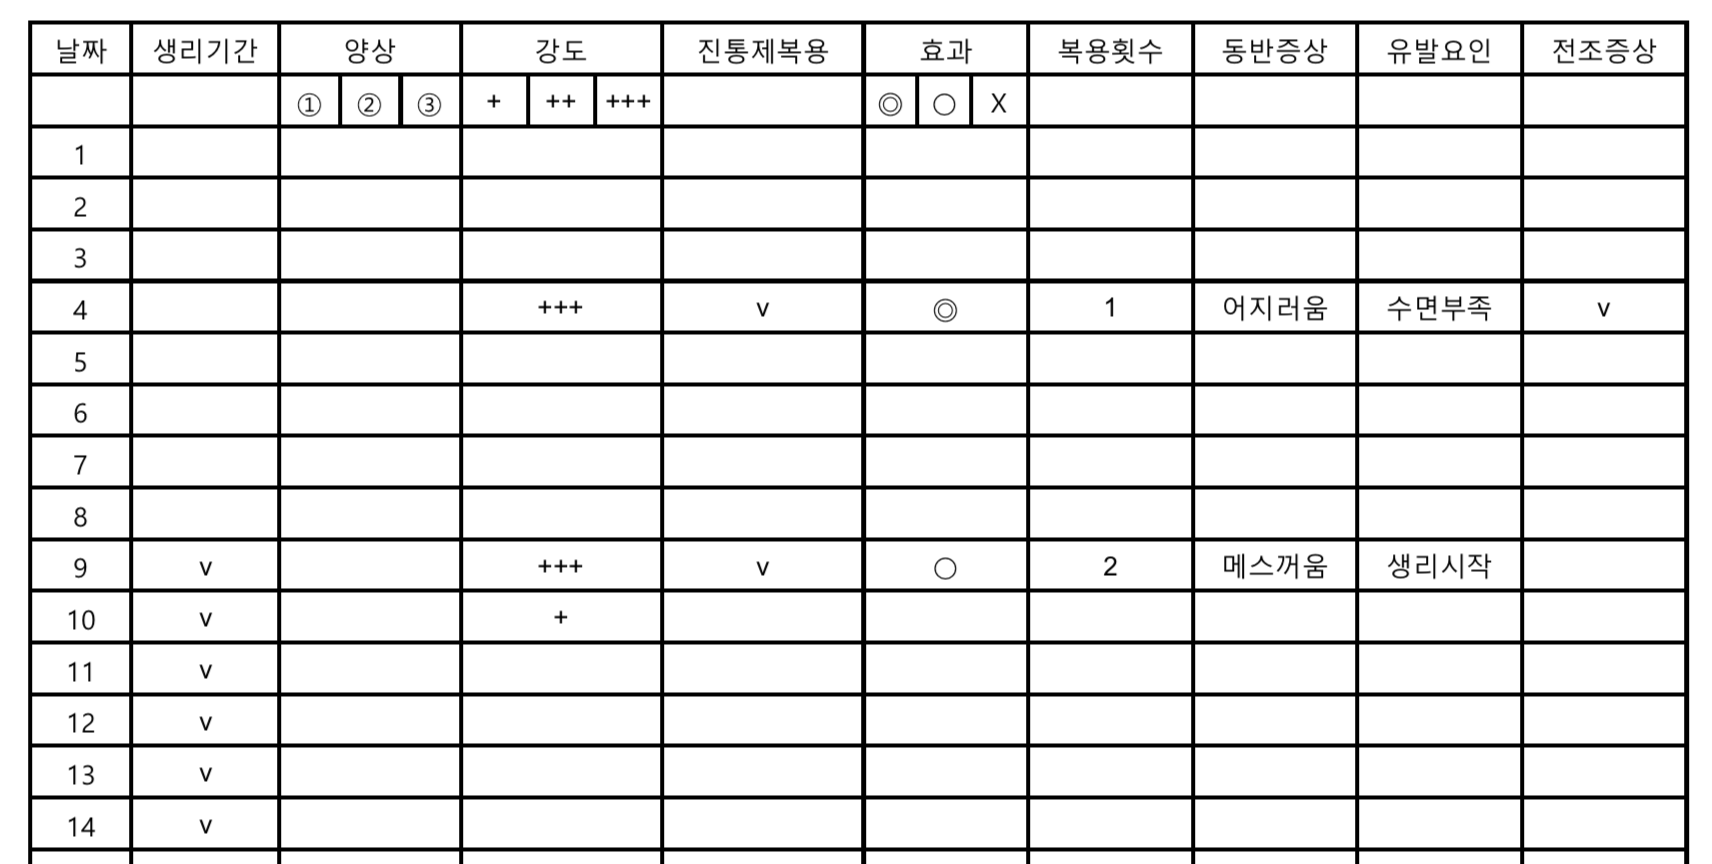
\includegraphics{static/DiaryExample.png}
\caption{두통일기의 예시}
\end{figure}

\hypertarget{section-22}{%
\chapter{삽화편두통 예방약물의 용량, 부작용 및 금기사항}\label{section-22}}

\hypertarget{section-23}{%
\section{일반적인 용량 및 흔한 부작용}\label{section-23}}

\begin{longtable}{lllllllll}
\toprule
약물 & 용량범위 & 부작용\\
\midrule
베타차단제 &  & \\
프로프라놀롤 & 10-80mg b.i.d. & 피로, 어지럼, 우울, 생생한 꿈\\
메토프롤롤 & 25-100mg b.i.d. & 피로, 어지럼, 우울, 생생한 꿈\\
아테놀롤 & 50-200mg per day & 피로, 어지럼, 우울, 생생한 꿈, 숨참, 서맥, 심계항진, 구역\\
나돌롤 & 40-160 per day & 피로, 어지럼, 우울, 생생한 꿈, 숨참, 서맥, 심계항진, 구역\\
\addlinespace
네비볼롤 & 2.5-5mg q.d. & 두통, 어지럼, 감각이상, 악몽, 위장장애, 호흡곤란, 가려움, 부종\\
비소프롤롤 & 1.25-10mg q.d. & 서맥, 두통, 어지럼, 오심, 구토, 설사, 변비, 피로\\
핀돌롤 & 5-30mg qd or b.i.d. & 불면증, 어지럼, 피로, 악몽, 소화불량, 호흡곤란, 근육통, 관절통\\
칼슘통로차단제 &  & \\
플루나리진 & 5-10mg q.d. or b.i.d. & 체중증가, 졸림, 입마름, 어지럼, 저혈압, 우울\\
\addlinespace
신나리진 & 25mg b.i.d. & 체중증가, 졸림, 입마름, 어지럼, 저혈압, 우울\\
베라파밀 & 80-640mg q.d. or b.i.d. & 심계항진, 부종, 부정맥, 발진\\
니카르디핀 & 20-40mg b.i.d. & 변비, 안면홍조, 무력, 두통, 근육통, 진전, 어지럼\\
니페디핀 & 15-60mg per day & 변비, 안면홍조, 무력, 두통, 근육통, 진전, 어지럼\\
니모디핀 & 30mg t.i.d. & 위장장애, 두통, 현기증, 졸음, 진전\\
\addlinespace
ACEI or ARB &  & \\
칸데사르탄 & 4-16mg q.d.(32mg까지) & 저혈압, 울혈심부전의 악화\\
리시노프릴 & 10-20mg q.d. & 어지럼, 두통, 기침, 피로, 근육경련, 설사, 저혈압\\
텔미사르탄 & 40-80mg q.d. & 고칼륨혈증, 어지럼, 저혈압, 발진, 근육통\\
항우울제 &  & \\
\addlinespace
아미트리프틸린 & 2.5-50mg q.d. & 체중증가, 변비, 무력증, 어지럼, 졸림, 피로, 시야흐림, 입마름\\
벤라팍신 & 37.5 - 150mg q.d. & 졸림, 불면, 어지럼, 두통, 구역, 입마름, 불안, 성기능장애\\
플루옥세틴 & 10-80mg q.d. & 무력, 구역, 설사, 불면, 식욕부진, 발기부전, 떨림, 불안, 초조\\
노르트리프틸린 & 25-150mg/d (노인감량) & 체중증가, 변비, 무력, 어지럼, 졸림, 피로, 시야흐림, 입마름\\
뇌전증약 &  & \\
\addlinespace
토피라메이트 & 12.5-150mg per day & 감각이상, 체중감소, 기억장애\\
디발프로엑스나트륨 & 250-1500mg per day & 구역, 체중증가, 떨림, 탈모, 졸림, 어지럼, 구토, 약물상호작용\\
발프로산 & 300-1000mg b.i.d. & 구역, 체중증가, 떨림, 탈모, 졸림, 어지럼, 구토, 약물상호작용\\
가바펜틴 & 100-600mg t.i.d. & 말초부종, 어지럼, 졸림, 실조증, 체중증가\\
레베티라세탐 & 250-1000mg b.i.d. & 무력증, 피로, 졸음, 어지럼, 근육통, 복시, 발진, 기침\\
\addlinespace
조니사미드 & 100-600mg/d & 체중감소, 복시/시각장애, 졸림, 의욕저하\\
\bottomrule
\end{longtable}

\hypertarget{section-24}{%
\section{금기사항}\label{section-24}}

\begin{longtable}{llllll}
\toprule
약물 & 금기사항\\
\midrule
베타차단제 & \\
프로프라놀롤 & 심한 천식, 당뇨, 말초혈관병, 심장전도장애, 울혈성심부전\\
메토프롤롤 & 심한 천식, 당뇨, 말초혈관병, 심장전도장애, 울혈성심부전\\
아테놀롤 & 심한 천식, 당뇨, 말초혈관병, 심장전도장애, 울혈성심부전, 치료안된 크롬친화성세포종\\
나돌롤 & 심한 천식, 당뇨, 말초혈관병, 심장전도장애, 울혈성심부전, 모노아민산화효소억제제 사용(2주이내)\\
\addlinespace
네비볼롤 & 심한 천식, 말초혈관병, 심장전도장애, 울혈성심부전\\
비소프롤롤 & 서맥, 당뇨성 케토산증, 급성 심부전, 치료안된  크롬친화성세포종, 중증 천식/만성 폐색성 폐질환\\
핀돌롤 & 천식, 중증 심부전, 서맥, 부정맥, 임신, 수유\\
칼슘통로차단제 & \\
플루나리진 & 심한 우울, 파킨슨병 기타 피라미드외로 증상\\
\addlinespace
신나리진 & 심한 우울, 파킨슨병 기타 피라미드외로 증상\\
베라파밀 & 서맥, 심장전도장애, 동결절기능부전 증후군, 중증근무력증, 급성심근경색\\
니카르디핀 & 뇌출혈후 지혈 안된 상태, 급성뇌졸중 두개내압상승, 심근경색, 중증신질환, 대동맥판막협착증\\
니페디핀 & 대동맥판막협착증, 급성심근경색, 불안정형 협심증, 임신, 리팜피신 복용중\\
니모디핀 & 과민증, 임신, 수유부, 중증간질환, 항경련제, 리팜피신복용 중\\
\addlinespace
ACEI or ARB & \\
칸데사르탄 & 혈관부종병력, 임신, 수유\\
리시노프릴 & 선천성 또는 특발성혈관부종, 다른 sulfonamide유도약물에 대한 과민\\
텔미사르탄 & 혈관부종병력, 중증간질환, 임신, 수유\\
항우울제 & \\
\addlinespace
아미트리프틸린 & 심근경색 급성기, cisapride나 모노아민산화효소억제제 사용\\
벤라팍신 & 모노아민산화효소억제제 병용, 수유중인 여성 주의\\
플루옥세틴 & 모노아민산화효소억제제, thioridazine, pimozied등 병용\\
노르트리프틸린 & 심근경색후 급성회복기, cisapride 사용, 모노아민산화효소억제제 사용\\
뇌전증약 & \\
\addlinespace
토피라메이트 & 약물과민, 신장질환, 요로계 결석\\
디발프로엑스나트륨 & 간질환, 췌장염, 임신, 요소순환질환, 저혈소판증\\
발프로산 & 간질환, 췌장염, 임신, 요소순환질환, 저혈소판증\\
가바펜틴 & 중증신질환\\
레베티라세탐 & 중증신질환, 이전 과민반응병력\\
\addlinespace
조니사미드 & 약물과민, 신장질환, 요로계 결석\\
\bottomrule
\end{longtable}

\hypertarget{section-25}{%
\chapter{편두통 진단기준}\label{section-25}}

\hypertarget{korean-version-of-the-international-classification-of-headache-disorders-3rd-edition}{%
\subsection*{Korean Version of The International Classification of Headache Disorders, 3rd Edition}\label{korean-version-of-the-international-classification-of-headache-disorders-3rd-edition}}
\addcontentsline{toc}{subsection}{Korean Version of The International Classification of Headache Disorders, 3rd Edition}

\hypertarget{section-26}{%
\section*{무조짐 편두통}\label{section-26}}
\addcontentsline{toc}{section}{무조짐 편두통}

A. 진단기준 B-D를 충족하는 발작이 최소한 5번

B. 두통 발작이 4-72시간 지속(치료하지 않거나 치료가 제대로 되지 않았을 경우)

C. 다음 네 가지 두통의 특성 중 최소한 두 가지:

\begin{enumerate}
\def\labelenumi{\arabic{enumi}.}
\tightlist
\item
  편측위치
\item
  박동양상
\item
  중등도 또는 심도의 통증 강도
\item
  일상신체활동(걷거나 계단을 오르는 등)에 의해 악화 또는 이를 회피하게 됨
\end{enumerate}

D. 두통이 있는 동안 다음 중 최소한 한 가지:

\begin{enumerate}
\def\labelenumi{\arabic{enumi}.}
\tightlist
\item
  구역 그리고/또는 구토
\item
  빛공포증과 소리공포증
\end{enumerate}

E. 다른 ICHD-3 진단으로 더 잘 설명되지 않음.

\hypertarget{section-27}{%
\section*{조짐 편두통}\label{section-27}}
\addcontentsline{toc}{section}{조짐 편두통}

A. 진단기준 B와 C를 충족하며 최소한 2번 발생하는 발작

B. 완전히 가역적인 다음의 조짐증상 중 한 가지 이상:

\begin{enumerate}
\def\labelenumi{\arabic{enumi}.}
\tightlist
\item
  시각
\item
  감각
\item
  말 그리고/또는 언어(speech and/or language)
\item
  운동
\item
  뇌간
\item
  망막
\end{enumerate}

C. 다음 여섯 가지 특성 중 최소한 세 가지:

\begin{enumerate}
\def\labelenumi{\arabic{enumi}.}
\tightlist
\item
  최소한 한 가지 조짐증상이 5분 이상에 걸쳐 서서히 발생
\item
  두 가지 이상의 증상이 연속해서 발생함
\item
  각 조짐증상은 5-60분 동안 지속
\item
  최소한 한 가지 조짐증상은 편측
\item
  최소한 한 가지 조짐증상은 양성 증상
\item
  조짐이 두통과 동반되거나, 또는 조짐 60분 이내에 두통이 따라 나타남
\end{enumerate}

D. 다른 ICHD-3 진단으로 더 잘 설명되지 않음.

\hypertarget{section-28}{%
\chapter{지침 개발 과정}\label{section-28}}

\hypertarget{section-29}{%
\section{이해당사자의 참여}\label{section-29}}

\hypertarget{section-30}{%
\subsection{지침 제정 참여자 및 역할}\label{section-30}}

\hypertarget{section-31}{%
\subsubsection*{운영위원회}\label{section-31}}
\addcontentsline{toc}{subsubsection}{운영위원회}

\begin{itemize}
\item
  위원장: 인제대학교 정재면
\item
  간사: 중앙대학교 박광열
\item
  역할

  \begin{itemize}
  \tightlist
  \item
    진료지침 개발 기획 및 개발 방법 결정
  \item
    진료지침 검색과 선별, 평가 등 상세 수용개작 과정에 대한 전체 방법론 마련
  \item
    실무위원회 자문 및 개발 과정 검토
  \item
    진료지침의 보급 및 실행 전략 마련
  \end{itemize}
\end{itemize}

\hypertarget{section-32}{%
\subsubsection*{자문위원회}\label{section-32}}
\addcontentsline{toc}{subsubsection}{자문위원회}

\begin{itemize}
\item
  을지대학교 김병건
\item
  연세대학교 김원주
\item
  역할

  \begin{itemize}
  \tightlist
  \item
    실무위원회 자문 및 개발 과정 검토
  \end{itemize}
\end{itemize}

\hypertarget{section-33}{%
\subsubsection*{외부자문그룹}\label{section-33}}
\addcontentsline{toc}{subsubsection}{외부자문그룹}

\begin{itemize}
\item
  순천향대학교 이유경
\item
  한국보건의료연구원 박동아
\item
  역할

  \begin{itemize}
  \tightlist
  \item
    실무위원회 자문 및 개발 과정 검토
  \end{itemize}
\end{itemize}

\hypertarget{section-34}{%
\subsubsection*{실무위원회및 근거평가그룹}\label{section-34}}
\addcontentsline{toc}{subsubsection}{실무위원회및 근거평가그룹}

\begin{itemize}
\tightlist
\item
  분당제생병원 김병수
\item
  경북대학교 서종근
\item
  한림대학교 손종희
\item
  이화여자대학교 송태진
\item
  성균관대학교 이미지
\item
  성균관대학교 정필욱
\item
  한국보건의료연구원 최미영
\item
  전주예수병원 최윤주
\end{itemize}

\hypertarget{section-35}{%
\subsection{이해관계 선언}\label{section-35}}

운영위원회 및 실무위원회의 모든 위원은 자문료, 연구비, 지적재산권등의 재정적 이해상충, 지적이해상충, 그리고 개인적 이해상충을 문서로 공개하였다.

\hypertarget{section-36}{%
\subsection{운영}\label{section-36}}

\hypertarget{section-37}{%
\subsubsection*{합의원칙의 결정}\label{section-37}}
\addcontentsline{toc}{subsubsection}{합의원칙의 결정}

\begin{itemize}
\tightlist
\item
  토론
\item
  델파이 방식을 통한 합의
\end{itemize}

\hypertarget{section-38}{%
\subsubsection*{저자원칙의 결정}\label{section-38}}
\addcontentsline{toc}{subsubsection}{저자원칙의 결정}

\begin{itemize}
\tightlist
\item
  최종보고서: 정재면
\item
  저자포함: 개발그룹전체
\end{itemize}

\hypertarget{section-39}{%
\section{지침이 다루는 인구 집단}\label{section-39}}

\begin{itemize}
\tightlist
\item
  성인 삽화편두통 환자(남녀 모두, 동반질환 포함)
\item
  소아는 제외
\item
  만성편두통 환자 제외
\end{itemize}

\hypertarget{section-40}{%
\section{지침 사용 대상자}\label{section-40}}

국내에서 편두통 환자를 진료하는 모든 임상의사

\hypertarget{section-41}{%
\section{지침의 범위와 목적}\label{section-41}}

임상의사가 편두통 환자를 진료할 때 표준화된 삽화편두통 환자의 예방약물 사용을 제시한다.

\hypertarget{section-42}{%
\section{지침의 목적}\label{section-42}}

본 지침은 국내 임상 상황에서 성인 편두통 환자들을 진료하는 모든 임상의들에게 삽화편두통의 예방약물에 대한 표준화된 지침을 제시함으로써, 이에 대한 정확한 이해 및 효율적인 치료를 증진시킬 목적으로 개발되었다.

\hypertarget{section-43}{%
\section{외부 검토}\label{section-43}}

\hypertarget{section-44}{%
\subsection*{잠재적 승인기구}\label{section-44}}
\addcontentsline{toc}{subsection}{잠재적 승인기구}

\begin{itemize}
\tightlist
\item
  대한두통학회
\item
  대한신경과학회
\end{itemize}

\hypertarget{section-45}{%
\section{보급전략}\label{section-45}}

\begin{itemize}
\item
  대한두통학회와 대한신경과학회 홈페이지 게시
\item
  대한두통학회지와 대한신경과학회지에 게재
\item
  책으로 출판하여 학술대회에서 배포
\item
  Online book (gitbook)형태로도 게시
\end{itemize}

\hypertarget{section-46}{%
\section{갱신절차}\label{section-46}}

매년 초 편두통 예방약물 진료지침 개정위원회를 개최하고, 새로운 근거를 검토하여 갱신의 필요성과 여부를 결정할 예정

\hypertarget{section-47}{%
\section{편집의 독립성과 재정}\label{section-47}}

대한두통학회 편두통진료지침위원 구성원들간에 이해상충이나 잠재적인 이해관계는 없었다. 또한, 대한신경과학회와 대한두통학회외의 기관이나 단체로부터 재정 지원을 받지 않았다.

\hypertarget{section-48}{%
\chapter{범위결정과 핵심질문}\label{section-48}}

\hypertarget{section-49}{%
\section{범위결정}\label{section-49}}

\begin{itemize}
\item
  Population: Adult with frequent and/or moderate-to-severe episodic migraine
\item
  Intervention: Drug

  \begin{itemize}
  \tightlist
  \item
    Anti-epileptic drug
  \item
    Beta blocker/CCB/ARB/ACE
  \item
    Anti-Depressant
  \end{itemize}
\item
  Professional:

  \begin{itemize}
  \tightlist
  \item
    Primary care physician, Nurse, and healthcare professionals
  \end{itemize}
\item
  Outcome: The frequency of migraine prevention drug prescription as suggested
\item
  Healthcare setting: Primary care setting in Korea
\end{itemize}

\hypertarget{section-50}{%
\section{핵심질문}\label{section-50}}

\hypertarget{section-51}{%
\subsection{선정과정}\label{section-51}}

\begin{itemize}
\item
  핵심질문 및 관련 검색어를 실무위원회에서 일차적으로 작성후 개발위원회에서 취합하여 검토 후 최종 선정하였다.
\item
  진료지침의 최종 권고안은 핵심질문을 기반으로 도출하였다.
\item
  핵심질문은 대상 환자·인구집단(P, patient population), 중재법(I, intervention), 비교 중재법(C, comparator), 중재결과(O, outcome) 내용을 구체적으로 포함하였다.

  \begin{itemize}
  \tightlist
  \item
    대상 환자·인구집단: 대상 환자·인구집단의 연령, 성별, 임상적 특성 및 증상, 특정 질환에 대한 이력, 이전 치료 등의 구체적 특성을 하위집단 개념으로 최대한 구분하여 기술하였다.\\
  \item
    중재법: 대상 중재법을 편두통 예방약물의 기전에 따라 5개의 군으로 정의하였다.
  \item
    비교 중재법: 편두통 예방약물의 효과를 판정하기 위해 위약의 효과와 비교하였다. 핵심질문에 따라 포함되지 않는 경우도 있었다.
  \item
    중재결과: 예방 치료의 목적 대상이 되는 해당 중재법의 임상적 주요 결과(두통 발작 일수의 감소, 강도의 감소) 등을 기술하였다.
  \end{itemize}
\item
  검색어

  \begin{itemize}
  \tightlist
  \item
    핵심질문의 PICO에 해당하는 영문 검색어를 정리하였다.
  \item
    실무위원회에서 선정된 핵심질문 및 검색어는 아래와 같은 서식을 활용하여 정리하였으며, 관련 진료지침을 검색하기 위하여 정리된 결과물을 개발위원회에 제공하였다.
  \end{itemize}
\end{itemize}

\hypertarget{section-52}{%
\subsection{최종 선정된 핵심질문}\label{section-52}}

\begin{enumerate}
\def\labelenumi{\arabic{enumi}.}
\item
  Episodic migraine환자에서 예방치료를 고려해야 하는 요인들(두통빈도, 두 통강도, 환자의 선호도, ADL에 대한 영향 등)은 무엇인가?
\item
  예방치료를 진행중인 episodic migraine환자에서 치료의 중단은 어떻게 결 정해야 하는가?
\item
  Episodic migraine환자에서 예방치료로 베타차단제(beta blocker: propranolol 등)를 사용하는 것이 타약제, 위약 또는 치료하지 않는 것에 비해 두통의 완화에 효과적인가?
\item
  Episodic migraine환자에서 예방치료로 칼슘채널차단제(calcium channel blocker: flunarizine 등)를 사용하는 것이 타약제, 위약 또는 치료하지 않는 것에 비해 두통의 완화에 효과적인가?
\item
  Episodic migraine환자에서 예방치료로 안지오텐신전환효소억제제(angiotensin converting enzyme inhibitor)나 안지오텐신수용체차단제(angiotensin receptor blocker: candesartan 등)를 사용하는 것이 타약제, 위약 또는 치료 하지 않는 것에 비해 두통의 완화에 효과적인가?
\item
  Episodic migraine환자에서 예방치료로 항우울제(anti-depressant: amitryptiline 등)를 사용하는 것이 타약제, 위약 또는 치료하지 않는 것에 비해 두통의 완화에 효과적인가?
\item
  Episodic migraine환자에서 예방치료로 항경련제(anti-epileptic agent: divalproex sodium, sodium valproate, topiramate 등)를 사용하는 것이 타약제, 위약 또는 치료하지 않는 것에 비해 두통의 완화에 효과적인가?
\end{enumerate}

\hypertarget{section-53}{%
\chapter{개발의 엄격성}\label{section-53}}

\hypertarget{section-54}{%
\section{개발방법}\label{section-54}}

\begin{itemize}
\tightlist
\item
  \textbf{Adaptation}

  \begin{itemize}
  \tightlist
  \item
    2012 - 2017년까지의 진료지침 + 2012-2017년 사이 연구를 핵심질문별로 다시 검색
  \item
    그외 수기로 논문 추가 조사 (논문의 참고문헌등)
  \end{itemize}
\end{itemize}

\hypertarget{section-55}{%
\section{지침및 근거검색}\label{section-55}}

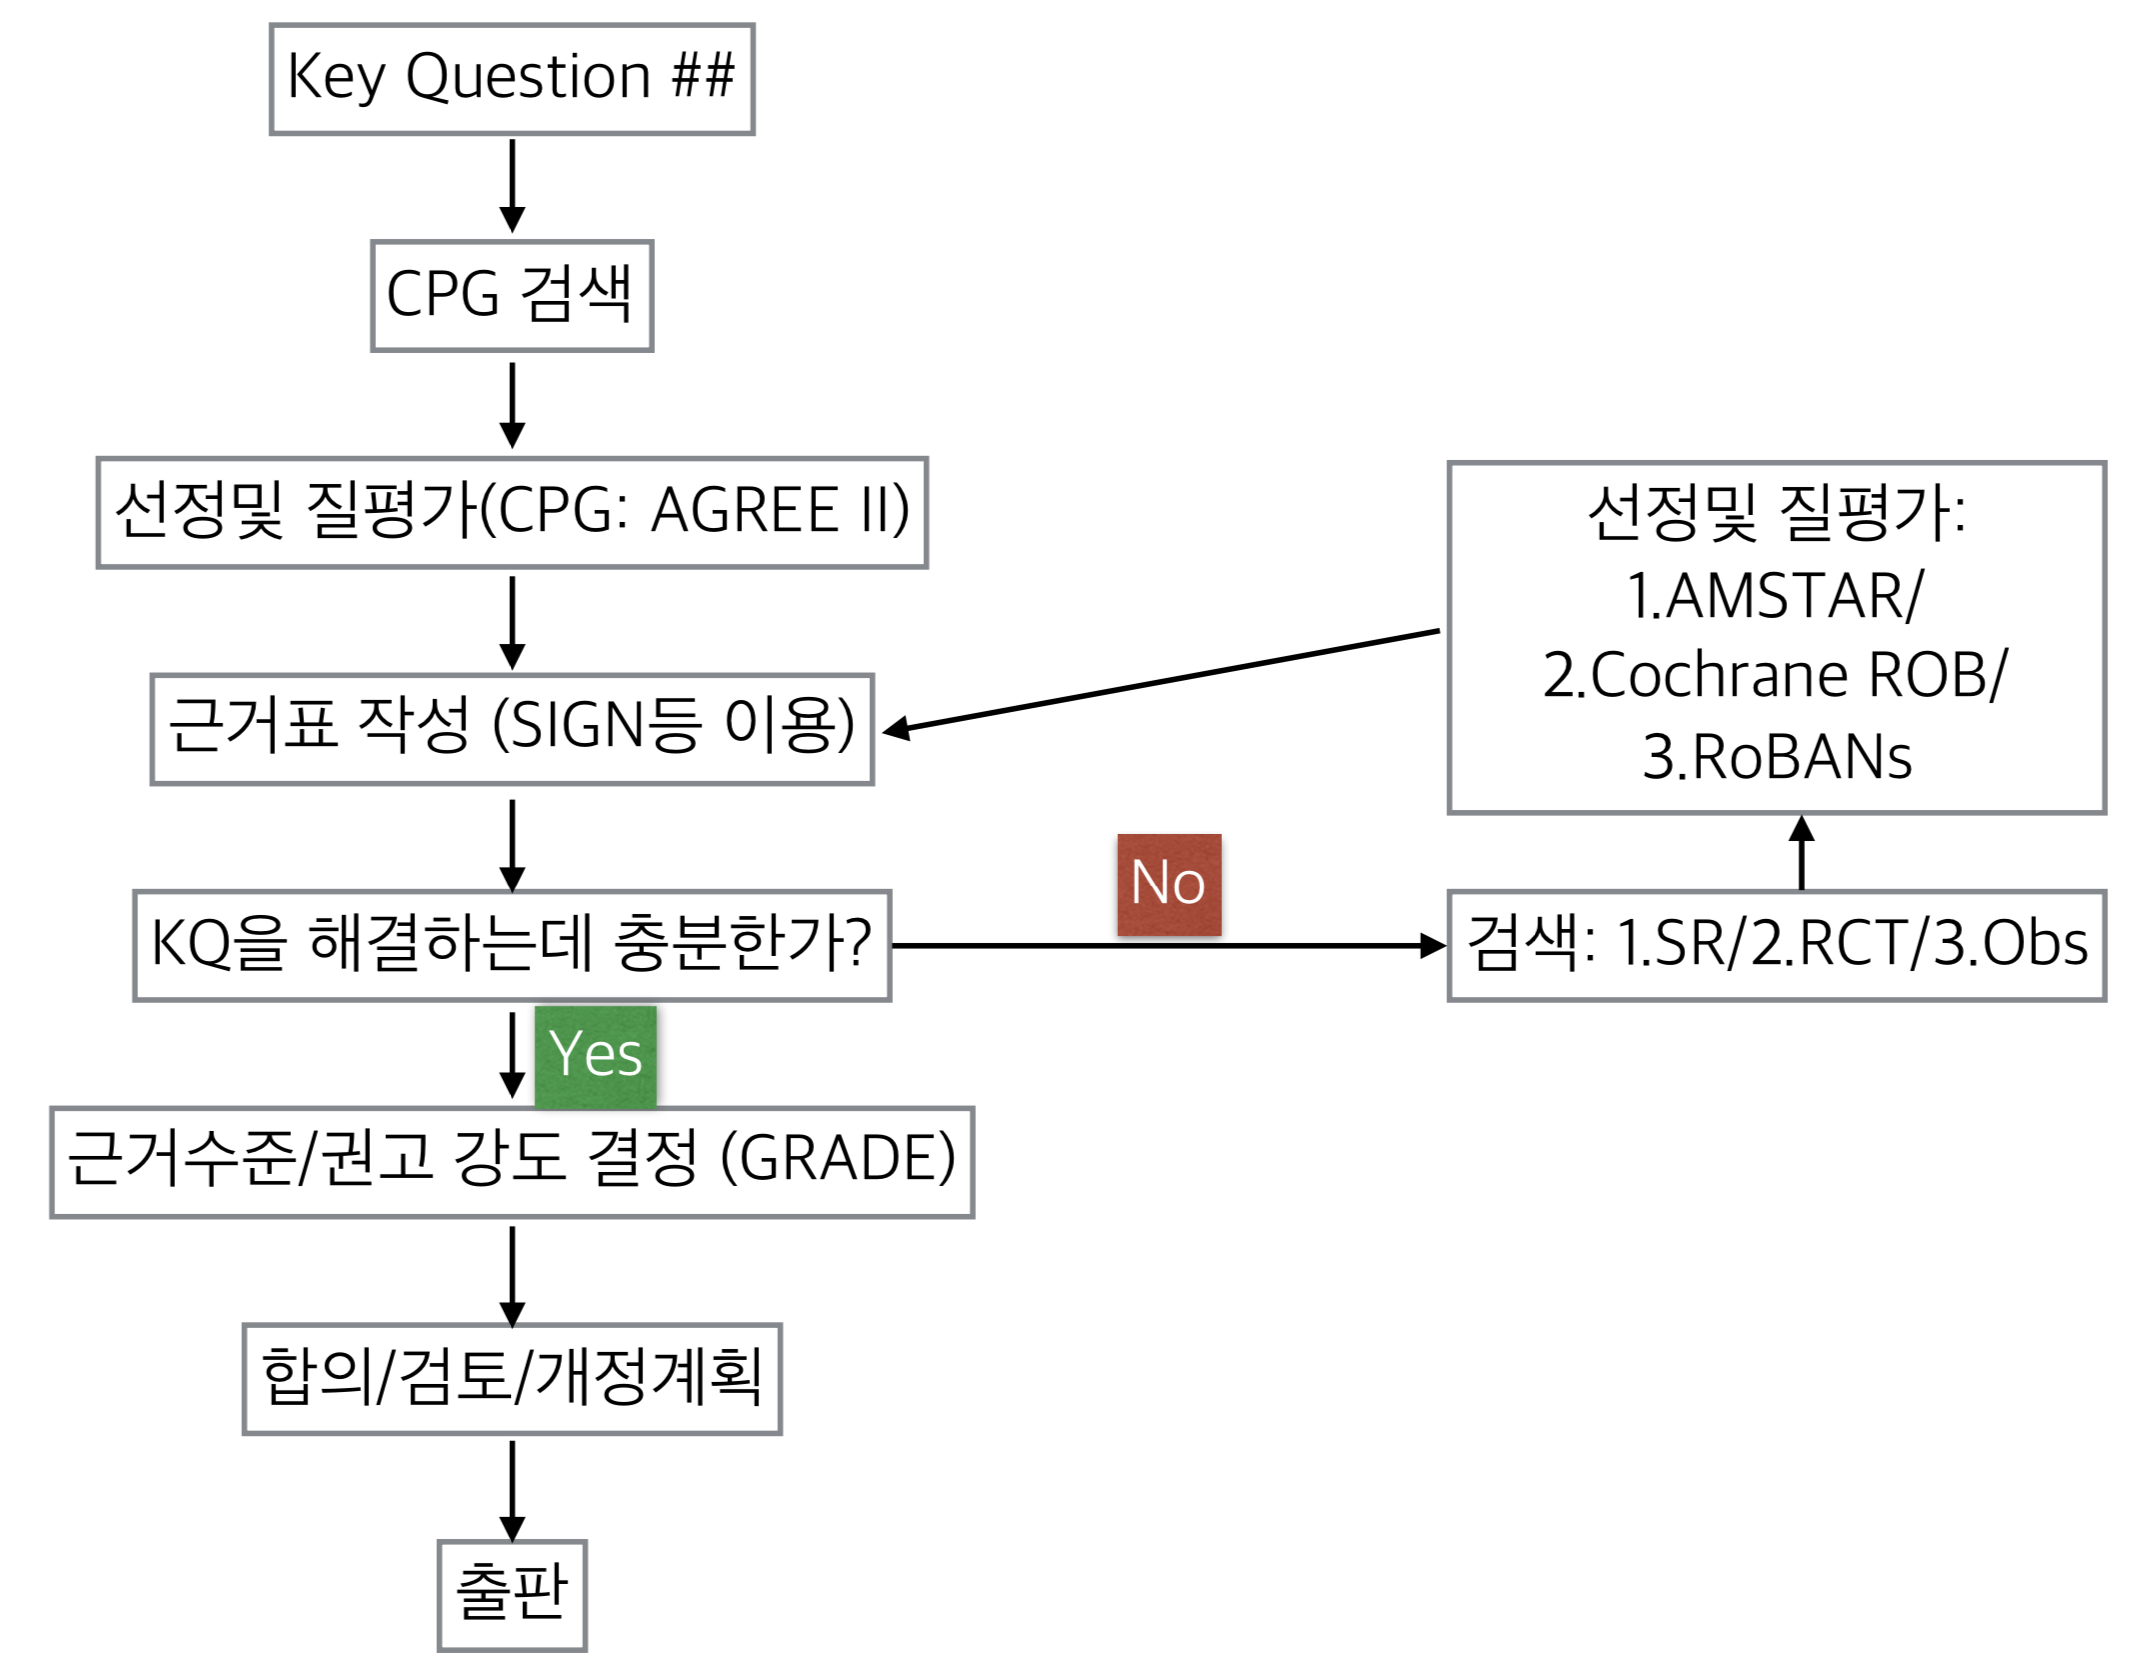
\includegraphics{static/SearchProcess.png}

\begin{itemize}
\tightlist
\item
  진료지침검색

  \begin{itemize}
  \tightlist
  \item
    정보원

    \begin{itemize}
    \tightlist
    \item
      National guideline clearinghouse
    \item
      Guideline international network
    \item
      Pubmed
    \item
      Google search
    \item
      KoMGI
    \item
      KoreaMed - KMBASE
    \end{itemize}
  \end{itemize}
\item
  근거검색

  \begin{itemize}
  \tightlist
  \item
    검색원

    \begin{itemize}
    \tightlist
    \item
      전자문헌검색: 상기 + Ovid DB(MEDLINE/EMBASE) Cochrane library
    \item
      수기검색 (gray literature)
    \end{itemize}
  \end{itemize}
\item
  검색 결과

  \begin{itemize}
  \tightlist
  \item
    \href{static/SearchingResult_\%20201710.pdf}{최신성 검색}: online only material

    \begin{itemize}
    \tightlist
    \item
      2012-2017년 10월까지 검색어, 검색결과
    \end{itemize}
  \end{itemize}
\end{itemize}

\hypertarget{section-56}{%
\section{검색된 진료지침및 연구결과 선별}\label{section-56}}

\begin{itemize}
\tightlist
\item
  선정 기준

  \begin{itemize}
  \tightlist
  \item
    핵실질문과 일치하는 PICO를 포함
  \item
    동료검토가 이루어 진것
  \item
    한국어 또는 영어로 출판된 것
  \item
    근거기반 방법론을 사용한 것
  \item
    2012년 이후 출판
  \end{itemize}
\end{itemize}

\hypertarget{section-57}{%
\section{검색된 진료지침및 연구결과 평가}\label{section-57}}

\begin{itemize}
\tightlist
\item
  진료지침은 AGREE-II를 이용하여 평가.
\item
  진료지침만으로 핵심질문을 답하는데 충분하지 않으면 체계적 문헌고찰, 무작위비교임상시험, 관찰연구등 순으로 추가 자료에 대해 질평가를 시행하고 근거표를 작성하였음.
\end{itemize}

\hypertarget{section-58}{%
\section{권고문 합의및 권고등급 결정}\label{section-58}}

\hypertarget{grade--}{%
\subsection*{근거수준과 권고등급의 평가: GRADE 방식 사용}\label{grade--}}
\addcontentsline{toc}{subsection}{근거수준과 권고등급의 평가: GRADE 방식 사용}

\hypertarget{section-59}{%
\subsubsection*{근거수준}\label{section-59}}
\addcontentsline{toc}{subsubsection}{근거수준}

근거수준(level of evidence)는 현재까지의 근거를 바탕으로 특정 중재의 효과에 대해 확신하는 정도를 말한다.

본 지침에서는 GRADE방식을 수정차용하여 아래와 같이 평가하였다.

\begin{itemize}
\tightlist
\item
  \textbf{높음}: 추정된 효과가 실제효과와 비슷할 것이라고 매우 확신한다.
\item
  \textbf{보통}: 추정된 효과가 실제 효과와 근접할 것이라고 확인한다. 하지만 상당히 다를 수 있는 가능성도 있다.
\item
  \textbf{낮음}: 추정된 효과는 실제효과와 아마도 상당히 다를지 모른다.
\item
  \textbf{매우 낮음}: 추정된 효과는 실제효과에 상당히 다를 가능성이 있다.
\item
  \textbf{전문가 의견}: 기존 근거가 별로 없으나 본 위원회 전문가의 공식적 합의 절차를 거쳐 현재 수준에서 임상적 적용을 하기에 적절함.
\end{itemize}

\hypertarget{section-60}{%
\subsubsection*{권고등급}\label{section-60}}
\addcontentsline{toc}{subsubsection}{권고등급}

권고등급(strength of recommendation)ʼ이란
권고 대상 환자에게 해당 중재를 시행하였을 때 위해(harm)보다 이득 (benefit)이 더 클 것으로 혹은 작을 것으로 확신하는 정도를 말한다.
권고등급은 일반적으로

\begin{enumerate}
\def\labelenumi{\arabic{enumi}.}
\tightlist
\item
  근거수준,
\item
  효과 크기(이득과 위해의 저울질)
\item
  가치와 선호도,
\item
  자원이용(비용)
\end{enumerate}

의 네 가지를 고려하여 결정한다.

본 지침에서는 Tools for GRADE를 사용하여 아래와 같이 평가하였다.

\begin{itemize}
\tightlist
\item
  \textbf{Strong for}: 강하게 권고, ``사용하는 것을 권고한다.''
\item
  \textbf{Weak for}: 약하게 권고, ``사용하는 것을 고려할 수 있다.''
\item
  \textbf{Weak against}: 약하게 권고하지 않음, ``사용하지 않을 것을 제안한다.''
\item
  \textbf{Strong aginst}: 강하게 권고하지 않음, ``사용하지 않을 것을 권고한다.''
\end{itemize}

\bibliography{book.bib,packages.bib}


\end{document}
